\documentclass[journal]{IEEEtran}
\usepackage[T1]{fontenc}
\usepackage{amsmath,amssymb}
\usepackage{graphicx}
\usepackage{tikz}
\usepackage{pgfplots}
\pgfplotsset{compat=1.18}
\usepackage{algorithm}
\usepackage{algorithmic}
\usepackage{booktabs}
\usepackage{multirow}
\usepackage{url}

\usetikzlibrary{arrows.meta, positioning, shapes.geometric, shapes.multipart, fit, calc, backgrounds, decorations.pathreplacing}

% ============================================================
% Unified IEEE Color Palette (colorblind-safe)
% ============================================================
\definecolor{cPrimary}{RGB}{0,101,189}     % IEEE blue
\definecolor{cSecondary}{RGB}{204,51,51}   % Accent red
\definecolor{cTertiary}{RGB}{0,128,0}      % Success green
\definecolor{cQuart}{RGB}{230,159,0}       % Highlight orange
\definecolor{cFifth}{RGB}{117,112,179}     % Phase purple
\definecolor{cSixth}{RGB}{0,158,115}       % Pipeline teal
\definecolor{cGray}{RGB}{128,128,128}      % Neutral
\definecolor{cBg1}{RGB}{219,234,254}       % Light blue bg
\definecolor{cBg2}{RGB}{254,226,226}       % Light red bg
\definecolor{cBg3}{RGB}{220,252,231}       % Light green bg
\definecolor{cBg4}{RGB}{254,243,199}       % Light orange bg
\definecolor{cBg5}{RGB}{237,233,254}       % Light purple bg
\definecolor{cBg6}{RGB}{207,250,254}       % Light teal bg
\definecolor{cBgLight}{RGB}{245,245,245}   % Very light gray

% ============================================================
% Unified TikZ Styles (IEEE-compliant, 5.5-7pt lines)
% ============================================================
\tikzset{
  font=\scriptsize,
  >=Stealth,
  line width=0.6pt,
  % Input/Output nodes
  io/.style={
    rectangle, rounded corners=2pt,
    draw=cPrimary, line width=0.7pt, fill=cBg1,
    minimum width=1.8cm, minimum height=0.55cm,
    align=center, font=\scriptsize\bfseries,
  },
  % Process nodes
  proc/.style={
    rectangle, rounded corners=1pt,
    draw=black, line width=0.5pt, fill=white,
    minimum width=1.8cm, minimum height=0.5cm,
    align=center, font=\scriptsize,
  },
  % Engine nodes
  engine/.style={
    rectangle, rounded corners=3pt,
    draw=#1, line width=0.8pt, fill=#1!8,
    minimum width=3.2cm, minimum height=1.0cm,
    align=center, font=\scriptsize\bfseries,
  },
  engine/.default=cPrimary,
  % Decision diamond
  decision/.style={
    diamond, aspect=2.2,
    draw=cQuart, line width=0.7pt, fill=cBg4,
    minimum width=1.6cm, minimum height=0.5cm,
    align=center, font=\scriptsize, inner sep=1pt,
  },
  % Phase label
  phase/.style={
    font=\scriptsize\bfseries, text=cPrimary,
  },
  % Arrows
  flow/.style={->, line width=0.6pt, black},
  flowThick/.style={->, line width=0.9pt, cPrimary},
  flowDashed/.style={->, dashed, line width=0.5pt, cGray},
  % Group box
  group/.style={
    rectangle, rounded corners=2pt,
    draw=#1, line width=0.5pt, dashed,
    fill=#1!4, inner sep=4pt,
  },
  group/.default=cGray,
  % Annotation
  annot/.style={font=\tiny\itshape, text=cGray, align=center},
  label/.style={font=\tiny, text=black, align=center},
}

\renewcommand{\algorithmicrequire}{\textbf{Input:}}
\renewcommand{\algorithmicensure}{\textbf{Output:}}

\begin{document}

\title{DEAC: A Defensive Ensemble Framework for\\Automatic Graph-Based Clustering of High-Dimensional Data}

\author{Author~Name%
\thanks{Author Name is with the Affiliation, City, Country
(e-mail: email@example.com).}%
\thanks{Manuscript received Month Day, Year; revised Month Day, Year.}}

\maketitle

% ============================================================
% ABSTRACT
% ============================================================
\begin{abstract}
Clustering high-dimensional data without a known cluster count remains an
open problem, and most graph-based methods inherit two weaknesses: they
commit to a single data representation, and they trust the partition that
maximizes an \emph{internal} quality score. We show that the second
assumption is unsafe---optimizing internal objectives (modularity,
silhouette) with a metaheuristic can \emph{degrade} external agreement
(ARI) on the majority of datasets, because internal and external quality
are misaligned. We therefore propose \textbf{DEAC} (Defensive Ensemble
Adaptive Clustering), built around two ideas. First, \emph{EMR-CGC}, a
multi-representation ensemble that runs Shared Nearest Neighbor (SNN)
graphs with Leiden community detection across five representations and
twelve configurations, then selects the best-scoring partition---turning
representation choice from a fixed decision into an automatic one. Second,
a three-layer adaptive \emph{QualityGate} that does not blindly trust any
optimized candidate but \emph{arbitrates} among them, defaulting to a fixed
baseline unless an engine scores higher on internal metrics. A complementary
DE-optimized engine (AMR-DE) is added for the specific dataset regimes
where parameter search helps. On 12 benchmarks ($n \in [178, 10992]$,
$d \in [9, 4096]$) DEAC lifts mean ARI by 13.1\% over the baseline and---when
every method must discover the cluster count itself---significantly
outperforms five classical methods (KMeans, Spectral, Agglomerative, GMM,
HDBSCAN) on 9 of 12 datasets (Holm-corrected Wilcoxon $p<0.05$; Friedman
$p{<}0.001$). Against four
modern deep-clustering methods (N2D, DEC, IDEC, DCN) that are each given the
true cluster count, an oracle over DEAC's engines matches the strongest (N2D)
while inferring the count itself; its label-free QualityGate is a deployable
approximation that recovers 75\% of the oracle's gain over the baseline.
\end{abstract}

\begin{IEEEkeywords}
Clustering, High-dimensional data, Graph-based clustering, Differential Evolution, Shared Nearest Neighbors, Leiden algorithm, UMAP, Ensemble clustering
\end{IEEEkeywords}

% ============================================================
% 1. INTRODUCTION
% ============================================================
\section{Introduction}

Clustering seeks to uncover hidden structure in data without class labels~\cite{jain2010data}. As samples and feature dimensions both grow, clustering high-dimensional data has grown harder~\cite{steinbach2004challenges}, and three concrete difficulties follow from that growth:

\begin{enumerate}
\item \textbf{Unknown cluster count.} Most methods (KMeans, Spectral, GMM) require the number of clusters $C$ as an input, which is rarely available in practice.
\item \textbf{Representation dependence.} Clustering quality depends heavily on the choice of dimensionality reduction---PCA, UMAP, or t-SNE---and no single choice is best across all datasets.
\item \textbf{Hyperparameter sensitivity.} Graph-based clustering involves four tightly coupled hyperparameters---$k$ (neighbors), $d'$ (dimensions), $q$ (pruning), $r$ (resolution)---whose best values differ markedly from one dataset to the next.
\end{enumerate}

Graph-based clustering addresses the first difficulty but inherits the other two. Methods in this family~\cite{schaeffer2007graph} build a similarity graph and apply community detection~\cite{blondel2008fast,traag2019louvain} to recover clusters of arbitrary shape with $C$ determined automatically. Their quality, however, still depends on the graph hyperparameters and on the representation used---gaps that an adaptive framework can close.

\textbf{Contributions.} Building on that observation, we propose DEAC (Defensive Ensemble Adaptive Clustering). This paper makes four contributions:

\begin{enumerate}
\item \textbf{An internal--external misalignment result.} We give empirical
evidence that metaheuristic optimization of internal clustering objectives
can reduce external accuracy: our DE-optimized engine, despite maximizing
modularity and silhouette, scores \emph{below} a fixed baseline in mean ARI
(0.521 vs.\ 0.574). This motivates arbitration over blind trust.

\item \textbf{Multi-representation SNN ensemble (EMR-CGC).} Rather than
committing to one representation, EMR-CGC selects the best-scoring partition
across five representations $\times$ twelve SNN+Leiden configurations, lifting
mean ARI to 0.644 and automatically recovering the cluster count.

\item \textbf{Adaptive QualityGate.} A three-layer, size-adaptive arbitrator
that defaults to the baseline unless an engine scores higher on internal
metrics, curbing---though not eliminating---the failures of any single
optimized engine.

\item \textbf{A complementary optimization engine and empirical study.}
AMR-DE adds coverage on the specific dataset regimes where parameter search
pays off (e.g.\ well-separated, moderate-$C$ data). We evaluate on 12
benchmarks with Wilcoxon, Friedman, and Nemenyi tests against five classical
baselines.
\end{enumerate}

The rest of the paper follows this order. Section~\ref{sec:related} surveys related work. Section~\ref{sec:method} details the DEAC framework. Section~\ref{sec:exp} reports the experiments. Section~\ref{sec:disc} discusses findings and limits; Section~\ref{sec:conc} concludes.

% ============================================================
% 2. RELATED WORK
% ============================================================
\section{Related Work}\label{sec:related}

We group prior work into six strands and close with DEAC's position in that space.

\subsection{Graph-Based Clustering}
Graph-based methods build a similarity graph and apply community detection. Louvain~\cite{blondel2008fast} maximizes modularity greedily but may return disconnected communities. Leiden~\cite{traag2019louvain} fixes that with a refinement phase that guarantees connectivity. Follow-up work has refined KNN-graph construction~\cite{brito1997connectivity} and sparsified edges through pruning~\cite{satuluri2011local}. Whichever detector is used, the input graph depends on a prior dimensionality reduction.

\subsection{Dimensionality Reduction}
PCA~\cite{jolliffe2002principal} is linear and misses manifold structure. UMAP~\cite{mcinnes2018umap} preserves both local and global structure and is generally stronger than t-SNE~\cite{van2008visualizing} for downstream clustering~\cite{becht2019dimensionality}. Its sensitivity to hyperparameters, however, is well documented---which again favors adaptive selection over fixed defaults. When adaptation is framed as optimization, metaheuristics become relevant.

\subsection{Metaheuristic Optimization for Clustering}
Differential Evolution (DE)~\cite{storn1997differential} has been used to tune clustering objectives~\cite{das2008automatic}. Grey Wolf Optimizer~\cite{mirjalili2014grey} with L\'{e}vy flights~\cite{yang2010nature} offers more aggressive exploration, and recent hybrids~\cite{faris2018grey} combine several heuristics---though they typically operate on a single representation. Representation diversity, which we pursue later, is rarely the primary target.

\subsection{SNN and DPC Approaches}
The Shared Nearest Neighbor (SNN) score~\cite{ertoz2003finding} sets edge weight from common neighbors rather than raw distance, which yields a more stable similarity. DPC-AKNN~\cite{wang2026density} pairs adaptive KNN with geodesic distance and reports ARI${>}0.95$ on small manifold datasets (${\leq}366$ samples), but still requires the true $C$ as input---a reliance it shares with the deep methods surveyed next.

\subsection{Deep Clustering}
A parallel line of work learns the representation and the clustering jointly. DEC~\cite{xie2016unsupervised} self-trains an autoencoder embedding with a KL objective; IDEC~\cite{guo2017improved} adds a reconstruction term, and DCN~\cite{yang2017towards} couples the autoencoder with $k$-means. N2D~\cite{mcconville2021n2d} instead clusters the UMAP manifold of an autoencoded embedding and is a strong, lightweight baseline. All of these, however, require the cluster count $C$ as input---the very assumption DEAC removes---which motivates our direct empirical comparison against them in \S\ref{sec:exp}.

\subsection{Ensemble Clustering}
Ensembles~\cite{strehl2002cluster} combine multiple partitions through co-association matrices~\cite{fred2005combining} or consensus voting~\cite{vega2011survey}. Most ensembles draw from a single representation, so partition diversity is bounded by that single view. These six strands together inform how DEAC is positioned.

\subsection{Positioning of DEAC}
Table~\ref{tab:related} compares the features that distinguish graph-clustering pipelines. DEAC is the only method that combines adaptive representation (AR), automatic $k$ (AK), hyperparameter optimization (HO), ensembling (EN), and a quality gate (QG).

\begin{table}[htbp]
\centering
\caption{Feature comparison with related methods.}
\label{tab:related}
\footnotesize
\setlength{\tabcolsep}{3pt}
\begin{tabular}{lccccc}
\toprule
Method & AR & AK & HO & EN & QG \\
\midrule
KMeans~\cite{lloyd1982least} & -- & -- & -- & -- & -- \\
Spectral Clustering~\cite{ng2001spectral} & -- & -- & -- & -- & -- \\
HDBSCAN~\cite{campello2013density} & -- & $\checkmark$ & -- & -- & -- \\
Louvain~\cite{blondel2008fast} & -- & $\checkmark$ & -- & -- & -- \\
Leiden~\cite{traag2019louvain} & -- & $\checkmark$ & -- & -- & -- \\
DEC~\cite{xie2016unsupervised} & -- & -- & $\checkmark$ & -- & -- \\
DPC-AKNN~\cite{wang2026density} & -- & -- & partial & -- & -- \\
Cluster Ensembles~\cite{strehl2002cluster} & -- & -- & -- & $\checkmark$ & -- \\
\textbf{DEAC (ours)} & $\checkmark$ & $\checkmark$ & $\checkmark$ & $\checkmark$ & $\checkmark$ \\
\bottomrule
\end{tabular}
\end{table}

% ============================================================
% 3. PROPOSED METHOD
% ============================================================
\section{Proposed Method: DEAC Framework}\label{sec:method}

\subsection{System Overview}

The DEAC framework is organized as four sequential layers (Fig.~\ref{fig:system}): an \emph{Input Layer} receiving raw data, a \emph{Preprocessing Layer} that caches multiple representations, an \emph{Engine Layer} where three clustering engines run in parallel, and an \emph{Arbitration Layer} in which the QualityGate selects the final output. Before examining each engine in turn, we describe the graph-clustering pipeline they share.

\begin{figure*}[!t]
\centering
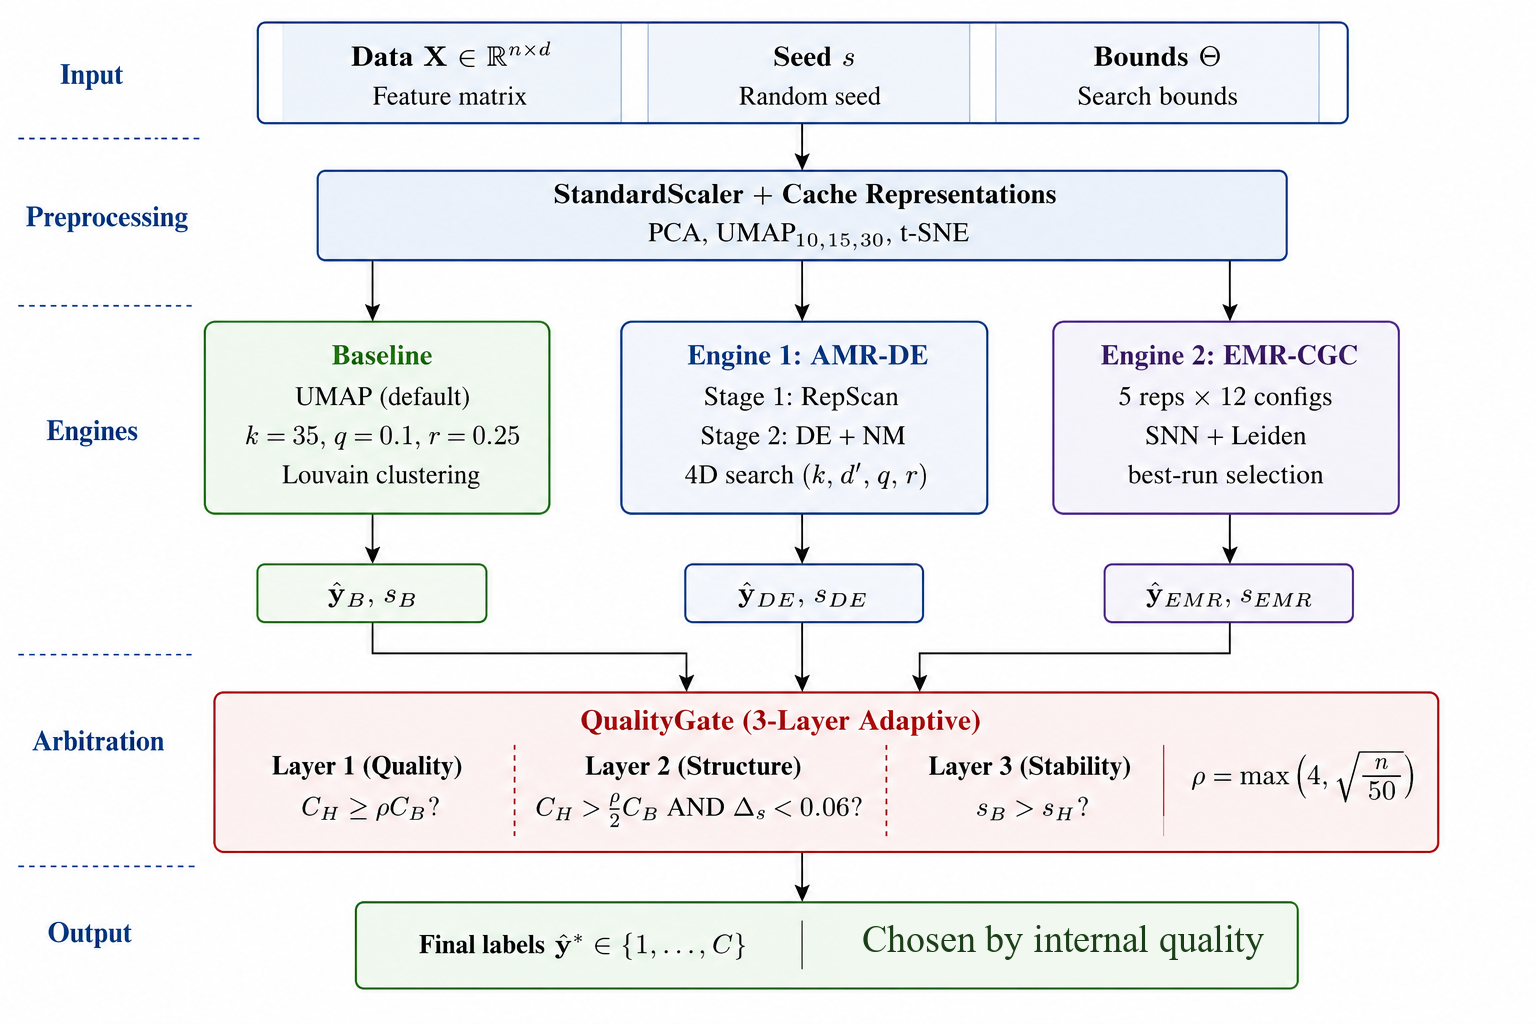
\includegraphics[width=0.65\textwidth]{figures/system_overview.png}
\caption{DEAC framework architecture. Four processing layers with three parallel clustering engines whose outputs are arbitrated by the QualityGate.}
\label{fig:system}
\end{figure*}

\subsection{Graph-Based Clustering Pipeline}

Both engines drive the same eight-step pipeline (Fig.~\ref{fig:pipeline}) that turns raw data $\mathbf{X} \in \mathbb{R}^{n \times d}$ into labels $\hat{\mathbf{y}}$. The engines differ only in how they score and search inside that pipeline, starting with AMR-DE.

\begin{figure*}[!t]
\centering
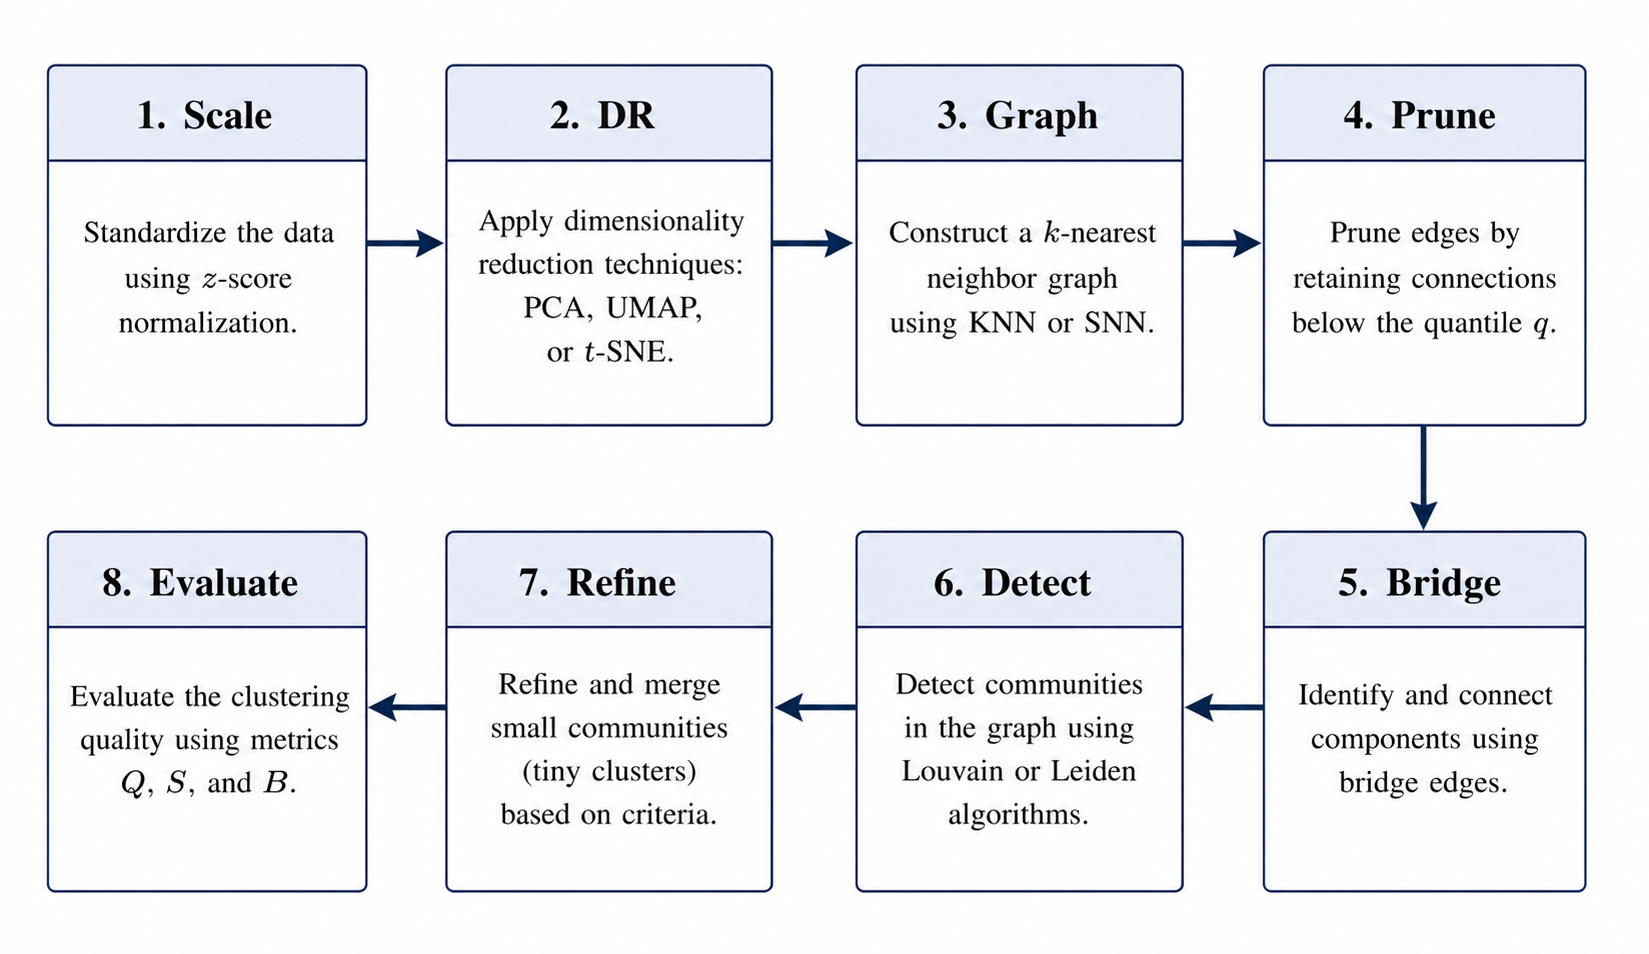
\includegraphics[width=0.65\textwidth]{figures/pipeline_overview.png}

\vspace{4pt}
{\tiny
$w_{ij}^{KNN} = (1+\cos(\mathbf{z}_i,\mathbf{z}_j))/2$ \quad\quad
$w_{ij}^{SNN} = |N_k(i)\cap N_k(j)|/k$ \quad\quad
$Q = \frac{1}{2m}\sum_{ij}\big[A_{ij}-\frac{d_i d_j}{2m}\big]\delta(c_i,c_j)$ \quad\quad
$S = \frac{1}{n}\sum_i \frac{b(i)-a(i)}{\max\{a(i),b(i)\}}$ \quad\quad
$B = H(\hat{\mathbf{y}})/\log C$}
\caption{Graph-based clustering pipeline (8 steps) shared by both engines. Key equations for KNN/SNN weighting and quality metrics are shown below.}
\label{fig:pipeline}
\end{figure*}

\subsection{Engine 1: AMR-DE}

AMR-DE (Fig.~\ref{fig:amrde}) runs in two stages. \textbf{Stage~1 (RepScan)} scores five representations with default graph parameters and selects the one that maximizes the composite score
\begin{equation}
s_{\text{rep}} = 0.30\,\text{MOD}_{01} + 0.40\,\text{SIL}_{01} + 0.30\,\text{CH}_{01},
\end{equation}
where MOD$_{01}$, SIL$_{01}$, and CH$_{01}$ are the $[0,1]$-normalized modularity, silhouette, and Calinski--Harabasz scores. \textbf{Stage~2 (Multi-Restart DE)} then optimizes four graph hyperparameters $\boldsymbol{\theta}=(k,d',q,r)$ on the fixed representation $\mathbf{Z}^*$. The fitness is a weighted sum of five quality metrics with penalties:
\begin{equation}
f(\boldsymbol{\theta}) = -\!\left(\sum_{m \in \mathcal{M}} w_m \cdot m_{01} - \text{penalties}\right),
\end{equation}
with $w_{\text{MOD}}{=}0.30$, $w_{\text{SIL}}{=}0.25$, $w_{\text{CH}}{=}0.20$, $w_{\text{DB}}{=}0.15$, $w_{\text{BAL}}{=}0.10$. AMR-DE commits to one representation; the second engine, by contrast, aggregates many.

\begin{figure*}[!t]
\centering
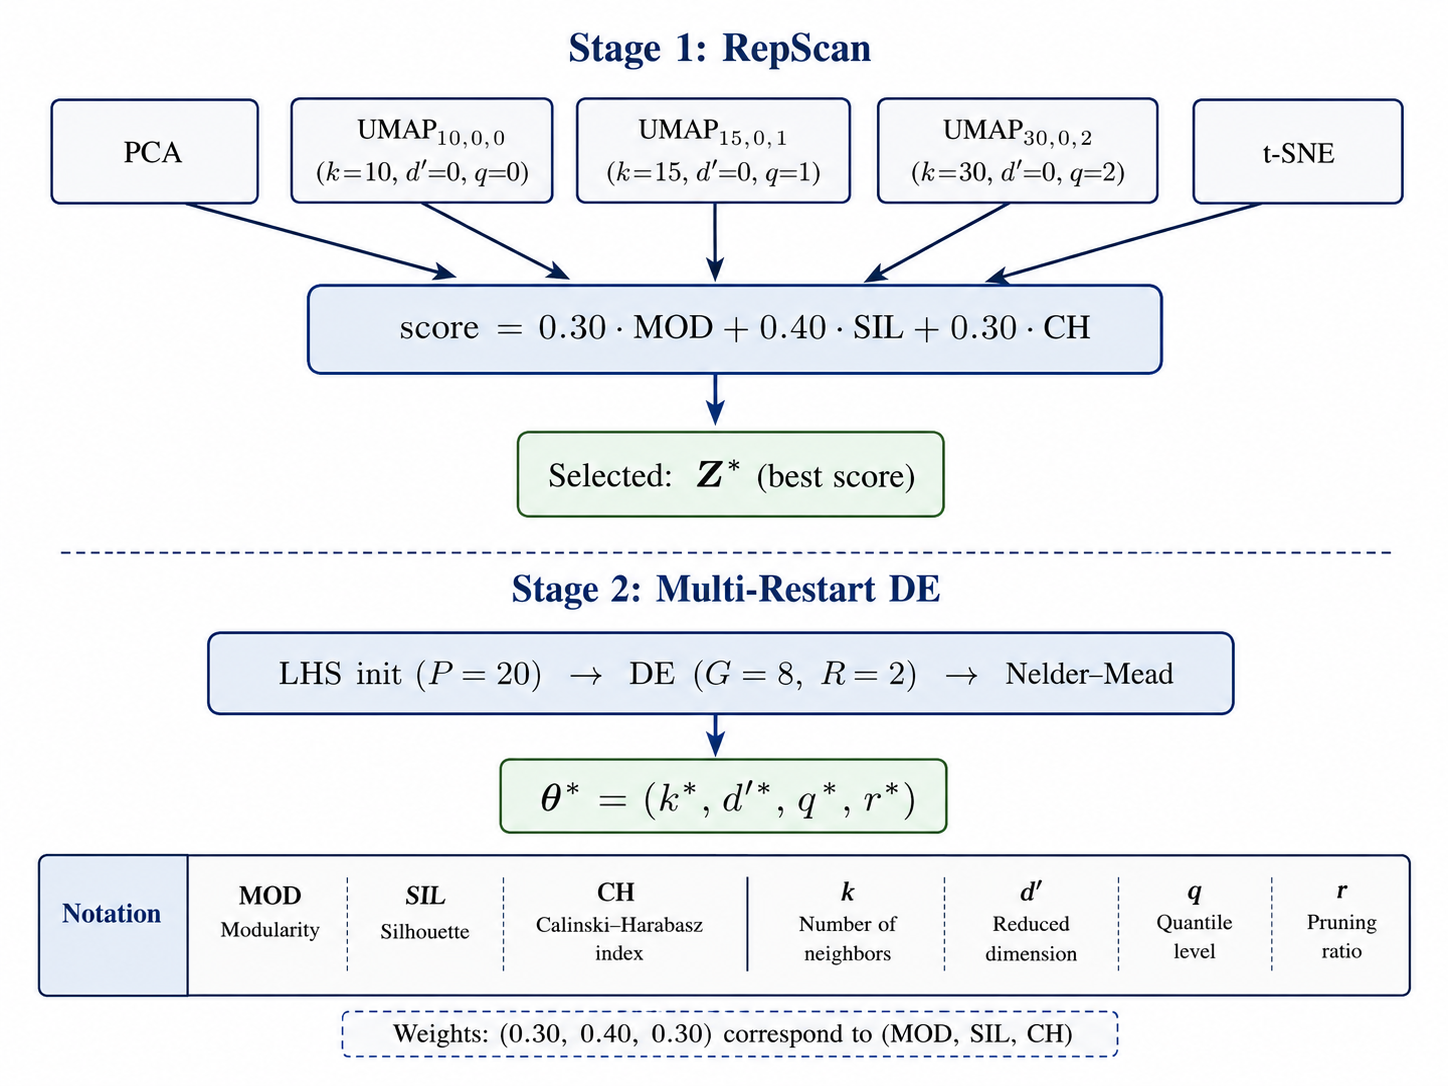
\includegraphics[width=0.65\textwidth]{figures/amrde_overview.png}
\caption{Engine~1 (AMR-DE): Stage~1 selects the best representation via RepScan; Stage~2 optimizes graph hyperparameters via multi-restart DE with Nelder--Mead refinement.}
\label{fig:amrde}
\end{figure*}

\subsection{Engine 2: EMR-CGC}

EMR-CGC (Fig.~\ref{fig:emrcgc}) produces 60 base clusterings---five representations $\times$ $|K|{=}4$ values of $k$ $\times$ $|R|{=}3$ resolutions---using Shared Nearest Neighbor (SNN) graphs and Leiden community detection. The SNN edge weight
\begin{equation}
w_{ij}^{\text{SNN}} = \frac{|N_k(i) \cap N_k(j)|}{k}
\end{equation}
captures structural similarity through shared neighbors and is less affected by noise and varying density than raw distance. The best base clustering is chosen by
\begin{equation}
s = 0.35\,\text{MOD}_{01} + 0.40\,\text{SIL}_{01} + 0.25\,\text{BAL}_{01}.
\end{equation}
With two independent candidates in hand, arbitration becomes the next question.

\begin{figure*}[!t]
\centering
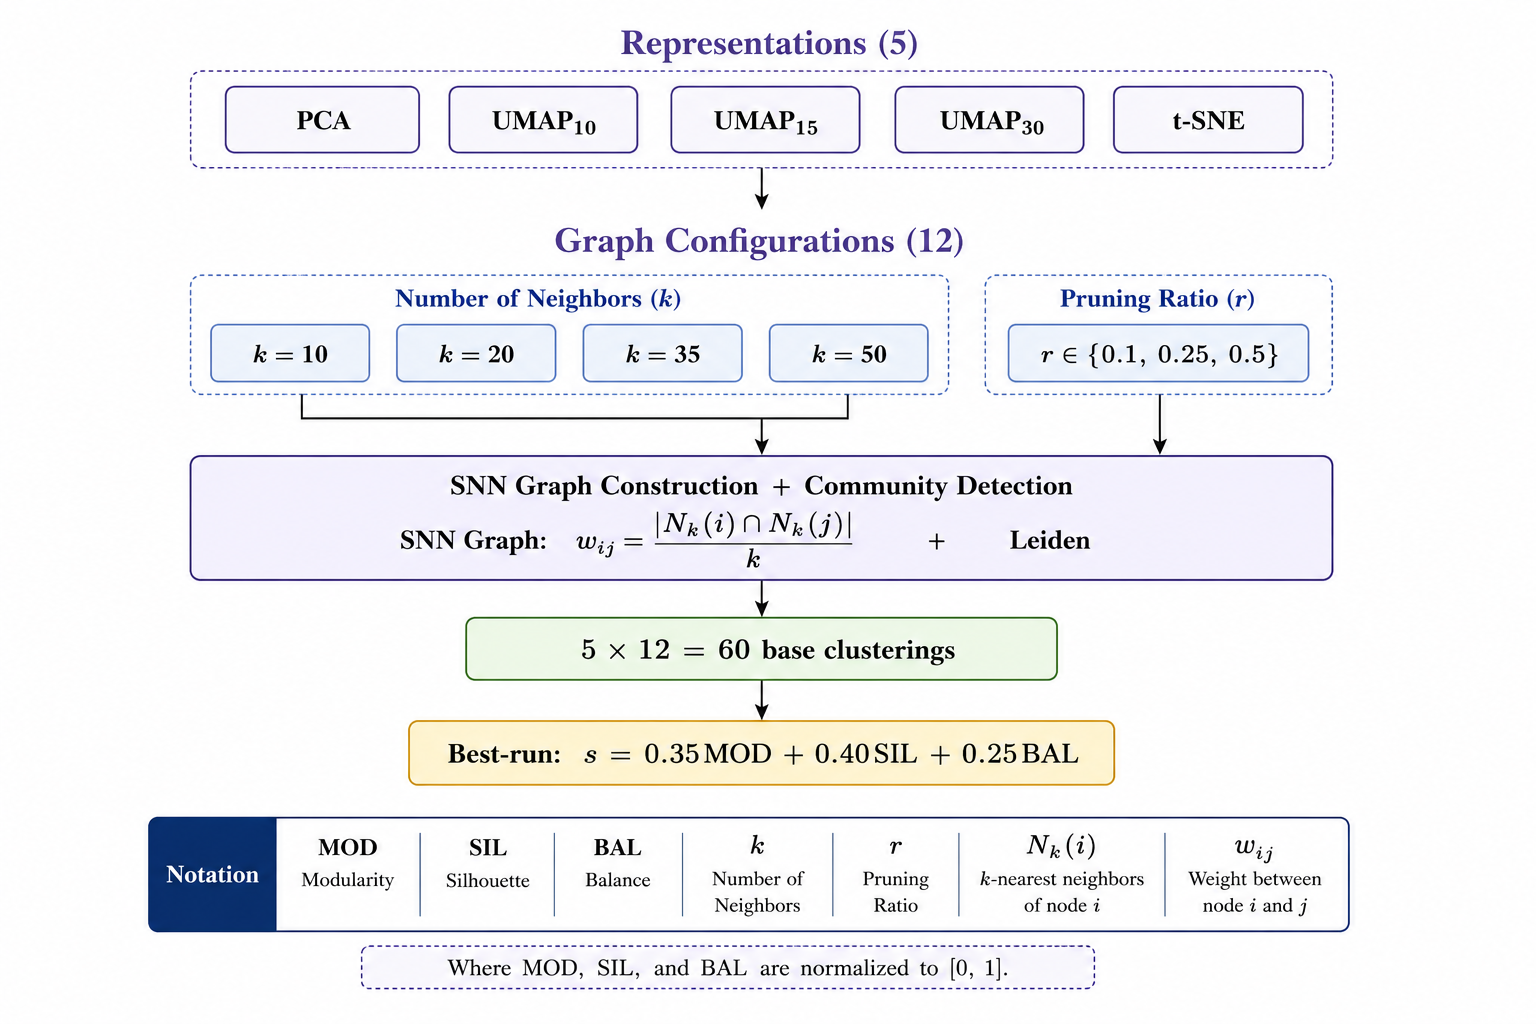
\includegraphics[width=0.65\textwidth]{figures/emrcgc_overview.png}
\caption{Engine~2 (EMR-CGC): Ensemble of 60 base clusterings from 5 representations $\times$ 12 graph configurations, using SNN graphs with Leiden community detection. Best run is selected by quality score.}
\label{fig:emrcgc}
\end{figure*}

\subsection{QualityGate}

The QualityGate (Fig.~\ref{fig:qg}) is a three-layer adaptive filter that selects $\max(\hat{\mathbf{y}}_B, \hat{\mathbf{y}}_{DE}, \hat{\mathbf{y}}_{EMR})$ using internal quality scores. Its C-ratio threshold $\rho = \max(4, \sqrt{n/50})$ is dataset-adaptive: larger datasets are permitted proportionally more clusters, while small ones are protected from over-fragmentation. Algorithms~\ref{alg:deac}--\ref{alg:emrcgc} give the full procedure.

\begin{figure}[!t]
\centering
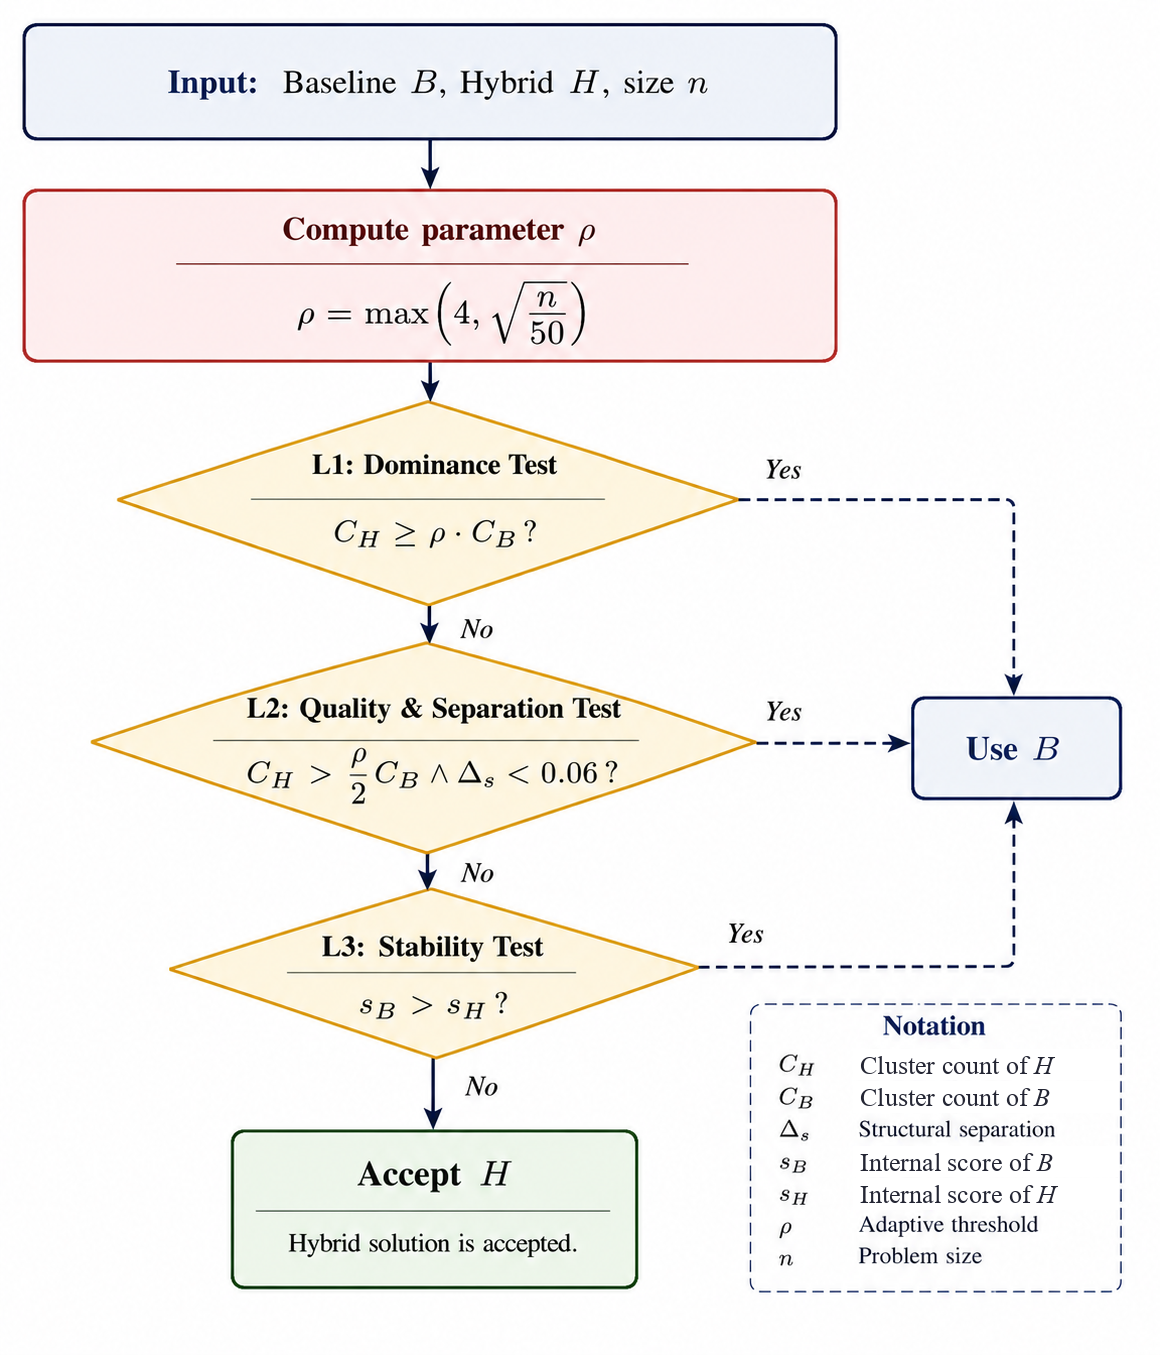
\includegraphics[width=\columnwidth]{figures/qg_overview.png}
\caption{QualityGate: three-layer adaptive protection. Layer~1 catches extreme over-fragmentation; Layer~2 catches moderate fragmentation with weak improvement; Layer~3 catches internal quality regression.}
\label{fig:qg}
\end{figure}

\subsection{Design Rationale}
\label{sec:rationale}

Two design choices warrant justification: the form of the threshold $\rho$ and the use of SNN rather than KNN edges.

\textbf{Why $\rho=\max(4,\sqrt{n/50})$.} Layer~1 must reject a partition only when its cluster count is implausibly large relative to the baseline. The number of clusters that can be \emph{statistically resolved} in a sample grows sublinearly with $n$: a classical rule of thumb places the maximum at $k_{\max}\approx\sqrt{n/2}$~\cite{mardia1979multivariate}. We therefore let the tolerated cluster-count ratio grow as $\sqrt{n}$ as well, so the gate's permissiveness tracks the rate at which genuine structure can appear. Writing the threshold as $\rho=\sqrt{n/c}$, the constant $c{=}50$ fixes the crossover with the floor at $n=50\cdot4^2=800$: below ${\sim}800$ samples the constant floor $\rho{=}4$ governs, above it the $\sqrt{n}$ term does (Table~\ref{tab:rho}). The floor of $4$ is deliberate---baselines routinely \emph{under}-segment (e.g.\ ISOLET baseline $C{=}8$ vs.\ $26$ true classes), so the gate must admit up to a $4\times$ increase to capture real fine structure, while still blocking the runaway fragmentation ($C_H\!\gg\!C_B$) that internal-metric optimization tends to produce. Layers~2--3 then catch the milder failure modes: moderate fragmentation paired with a negligible internal-score gain ($\Delta s<0.06$), and outright internal-quality regression. The thresholds are intentionally conservative; because the gate can only \emph{substitute the baseline}, an overly strict $\rho$ costs at most the engine's gain on a dataset, whereas an overly loose $\rho$ risks accepting a fragmented partition---an asymmetry that motivates erring toward the baseline.

% QualityGate over-fragmentation thresholds (rho = max(4, sqrt(n/50)))
\begin{table}[htbp]
\centering
\caption{Size-adaptive over-fragmentation threshold $\rho=\max(4,\sqrt{n/50})$ per dataset. Below the floor/$\sqrt{n}$ crossover ($n{=}800$) the constant floor governs; above it the $\sqrt{n}$ term governs.}
\label{tab:rho}
\footnotesize
\setlength{\tabcolsep}{4pt}
\begin{tabular}{lrcc}
\toprule
Dataset & $n$ & $\sqrt{n/50}$ & $\rho$ (regime) \\
\midrule
Wine         & 178   & 1.89  & 4.00 (floor) \\
Glass        & 214   & 2.07  & 4.00 (floor) \\
Olivetti     & 400   & 2.83  & 4.00 (floor) \\
CNAE-9       & 1080  & 4.65  & 4.65 ($\sqrt{n}$) \\
COIL-20      & 1440  & 5.37  & 5.37 ($\sqrt{n}$) \\
Optdigits    & 1797  & 5.99  & 5.99 ($\sqrt{n}$) \\
MFeat        & 2000  & 6.32  & 6.32 ($\sqrt{n}$) \\
Segmentation & 2310  & 6.80  & 6.80 ($\sqrt{n}$) \\
ISOLET       & 6006  & 10.96 & 10.96 ($\sqrt{n}$) \\
Satimage     & 6430  & 11.34 & 11.34 ($\sqrt{n}$) \\
USPS         & 9298  & 13.64 & 13.64 ($\sqrt{n}$) \\
PenDigits    & 10992 & 14.83 & 14.83 ($\sqrt{n}$) \\
\bottomrule
\end{tabular}
\end{table}


\textbf{Why SNN over KNN.} In high dimension, pairwise Euclidean distances concentrate---the contrast between nearest and farthest neighbors vanishes---so raw-distance edge weights become unreliable~\cite{beyer1999nearest}. The SNN weight $w_{ij}=|N_k(i)\cap N_k(j)|/k$ depends only on the \emph{overlap of neighbor sets}, a rank-based quantity that is far more stable than absolute distance under this concentration, and shared-neighbor similarities are known to mitigate the curse of dimensionality directly~\cite{houle2010shared}. This motivates SNN for the high-dimensional representations in EMR-CGC's ensemble; consistent with the theory, its measured benefit is concentrated on the highest-dimensional datasets, while it is neutral-to-negative elsewhere (\S\ref{sec:disc}).

\subsection{Algorithms}

The main DEAC algorithm and its two engines are presented in Algorithms~\ref{alg:deac}--\ref{alg:emrcgc}.

\begin{algorithm}[!t]
\caption{DEAC --- Main Algorithm}
\label{alg:deac}
\begin{algorithmic}[1]
\REQUIRE Data $\mathbf{X} \in \mathbb{R}^{n \times d}$, seed $s$
\ENSURE Cluster labels $\hat{\mathbf{y}}^*$
\STATE $\hat{\mathbf{y}}_B \leftarrow$ GraphCluster$(\mathbf{X},\text{UMAP}, k{=}35, q{=}0.1, r{=}0.25)$
\STATE $(\boldsymbol{\theta}^*, \text{rep}^*) \leftarrow$ AMR-DE$(\mathbf{X}, s)$ \COMMENT{Alg.~\ref{alg:amrde}}
\STATE $\hat{\mathbf{y}}_{DE} \leftarrow$ GraphCluster$(\mathbf{X}, \text{rep}^*, \boldsymbol{\theta}^*)$
\STATE $\hat{\mathbf{y}}_{EMR} \leftarrow$ EMR-CGC$(\mathbf{X}, s)$ \COMMENT{Alg.~\ref{alg:emrcgc}}
\STATE $\hat{\mathbf{y}}^* \leftarrow$ QualityGate$(\hat{\mathbf{y}}_B, \hat{\mathbf{y}}_{DE}, \hat{\mathbf{y}}_{EMR}, n)$
\RETURN $\hat{\mathbf{y}}^*$
\end{algorithmic}
\end{algorithm}

\begin{algorithm}[!t]
\caption{AMR-DE --- Engine 1}
\label{alg:amrde}
\begin{algorithmic}[1]
\REQUIRE Data $\mathbf{X}$, seed $s$
\ENSURE $(\boldsymbol{\theta}^*, \text{rep}^*)$
\STATE \textbf{Stage 1: RepScan}
\FOR{rep $\in\{$PCA, UMAP$_{10,15,30}$, t-SNE$\}$}
  \STATE $\mathbf{Z}_r \leftarrow$ ComputeRep$(\mathbf{X}, \text{rep}, s)$
  \STATE Score$_r \leftarrow 0.30\text{MOD}+0.40\text{SIL}+0.30\text{CH}$
\ENDFOR
\STATE rep$^* \leftarrow \arg\max$ Score$_r$; $\mathbf{Z}^* \leftarrow \mathbf{Z}_{rep^*}$
\STATE \textbf{Stage 2: Multi-Restart DE on $\mathbf{Z}^*$}
\FOR{restart $= 1$ to $R$}
  \STATE Init $P$ via Latin Hypercube Sampling
  \STATE Run DE for $G$ generations
  \STATE Refine best with Nelder--Mead
\ENDFOR
\RETURN $\arg\min$ fitness over restarts; rep$^*$
\end{algorithmic}
\end{algorithm}

\begin{algorithm}[!t]
\caption{EMR-CGC --- Engine 2}
\label{alg:emrcgc}
\begin{algorithmic}[1]
\REQUIRE Data $\mathbf{X}$, seed $s$
\ENSURE Cluster labels $\hat{\mathbf{y}}$
\STATE Reps $\leftarrow \{$PCA, UMAP$_{10,15,30}$, t-SNE$\}$
\STATE $K \leftarrow \{10, 20, 35, 50\}$; $R \leftarrow \{0.1, 0.25, 0.5\}$
\STATE results $\leftarrow \emptyset$
\FOR{rep $\in$ Reps}
  \STATE $\mathbf{Z} \leftarrow$ ComputeRep$(\mathbf{X}, \text{rep}, s)$
  \FOR{$k \in K$, $r \in R$}
    \STATE Build SNN graph with $w_{ij}=|N_k(i)\cap N_k(j)|/k$
    \STATE $\hat{\mathbf{y}}_i \leftarrow$ Leiden$(G_{\text{SNN}}, r)$
    \STATE $s_i \leftarrow 0.35\text{MOD}+0.40\text{SIL}+0.25\text{BAL}$
    \STATE results $\leftarrow$ results $\cup\,\{(\hat{\mathbf{y}}_i, s_i)\}$
  \ENDFOR
\ENDFOR
\RETURN $\arg\max_i s_i$
\end{algorithmic}
\end{algorithm}

% ============================================================
% 4. EXPERIMENTS
% ============================================================
\section{Experimental Evaluation}\label{sec:exp}

\subsection{Datasets}

DEAC is evaluated on 12 public benchmarks that span a wide range of $n$ and $d$ (Table~\ref{tab:datasets}). These datasets also determine the protocol below.

\begin{table}[htbp]
\centering
\caption{Benchmark datasets.}
\label{tab:datasets}
\footnotesize
\setlength{\tabcolsep}{4pt}
\begin{tabular}{lrrrl}
\toprule
Dataset & $n$ & $d$ & $C_{\text{true}}$ & Domain \\
\midrule
Wine         & 178   & 13   & 3  & Chemistry \\
Glass        & 214   & 9    & 6  & Material \\
Olivetti     & 400   & 4096 & 40 & Faces \\
CNAE-9       & 1080  & 856  & 9  & Text \\
COIL-20      & 1440  & 1024 & 20 & Images \\
Optdigits    & 1797  & 64   & 10 & Digits \\
MFeat        & 2000  & 649  & 10 & Digits \\
Segmentation & 2310  & 19   & 7  & Images \\
ISOLET       & 6006  & 617  & 26 & Speech \\
Satimage     & 6430  & 36   & 6  & Remote Sensing \\
USPS         & 9298  & 256  & 10 & Digits \\
PenDigits    & 10992 & 16   & 10 & Handwriting \\
\bottomrule
\end{tabular}
\end{table}

\subsection{Evaluation Protocol}

Three external validity indices are reported: Adjusted Rand Index (ARI)~\cite{hubert1985comparing}, Normalized Mutual Information (NMI)~\cite{strehl2002cluster}, and Clustering Accuracy (ACC)~\cite{yang2010image}. Unless noted, results are averaged over five fixed seeds ($1001$--$1005$) for reproducibility. DEAC is configured with AMR-DE ($G{=}8$, $P{=}20$, $R{=}2$) and EMR-CGC (60 base clusterings). The baseline is UMAP+Louvain with community-standard settings ($k{=}35$, $q{=}0.1$, resolution $0.25$)---a legitimate reference rather than a deliberately weakened one; indeed it is the single strongest engine on 1 of 12 datasets. With the protocol fixed, we turn to the headline results.

\subsection{Main Results}

Table~\ref{tab:main_results} compares the Baseline, the two engines in isolation, and DEAC under \emph{oracle} engine selection---the per-dataset best-ARI engine, which is an upper bound on what the label-free QualityGate can achieve. This oracle attains the best or tied-best ARI on all 12 datasets by construction, with a mean ARI of 0.649 against 0.574 for the baseline (+13.1\%). How much of this upper bound the deployable gate actually recovers---selecting without ground-truth labels---is quantified in \S\ref{sec:disc} (Table~\ref{tab:gate}). Fig.~\ref{fig:main_results} presents the evaluation in four complementary views: the dataset landscape~(a), the per-dataset ARI comparison~(b), the QualityGate activation per dataset~(c), and a multi-metric improvement heatmap sorted by $\Delta$ARI~(d). Internal comparison aside, the next question is how DEAC fares against established competitors.

\begin{table}[!t]
\centering
\caption{Main results. ARI across 12 datasets. Bold = best. DEAC here is the \emph{oracle} $\max$(Baseline, AMR-DE, EMR-CGC)---an upper bound; the deployable label-free gate is characterized in Table~\ref{tab:gate}.}
\label{tab:main_results}
\footnotesize
\setlength{\tabcolsep}{4pt}
\begin{tabular}{lcccc}
\toprule
Dataset & Baseline & AMR-DE & EMR-CGC & \textbf{DEAC} \\
\midrule
Wine         & 0.802 & 0.774 & \textbf{0.802} & \textbf{0.802} \\
Glass        & 0.150 & 0.147 & \textbf{0.174} & \textbf{0.174} \\
Olivetti     & 0.076 & 0.183 & \textbf{0.342} & \textbf{0.342} \\
CNAE-9       & 0.549 & 0.624 & \textbf{0.658} & \textbf{0.658} \\
COIL-20      & 0.622 & \textbf{0.777} & 0.762 & \textbf{0.777} \\
Optdigits    & \textbf{0.868} & 0.804 & 0.843 & \textbf{0.868} \\
MFeat        & 0.904 & 0.919 & \textbf{0.937} & \textbf{0.937} \\
Segment.     & 0.418 & 0.169 & \textbf{0.465} & \textbf{0.465} \\
Satimage     & 0.439 & 0.277 & \textbf{0.591} & \textbf{0.591} \\
ISOLET       & 0.457 & \textbf{0.498} & 0.473 & \textbf{0.498} \\
USPS         & 0.861 & 0.533 & \textbf{0.865} & \textbf{0.865} \\
PenDigits    & 0.736 & 0.550 & \textbf{0.810} & \textbf{0.810} \\
\midrule
\textbf{Mean} & 0.574 & 0.521 & 0.644 & \textbf{0.649} \\
\textbf{Best$^\dagger$} & 2/12 & 2/12 & 9/12 & \textbf{12/12} \\
\bottomrule
\end{tabular}

\vspace{2pt}
{\footnotesize $^\dagger$\,Number of datasets where the method attains the row-maximum ARI (ties counted). DEAC is the per-dataset maximum of the three source engines by construction.}
\end{table}

\begin{figure*}[!t]
\centering
\setlength{\tabcolsep}{3pt}
\begin{tabular}{cc}
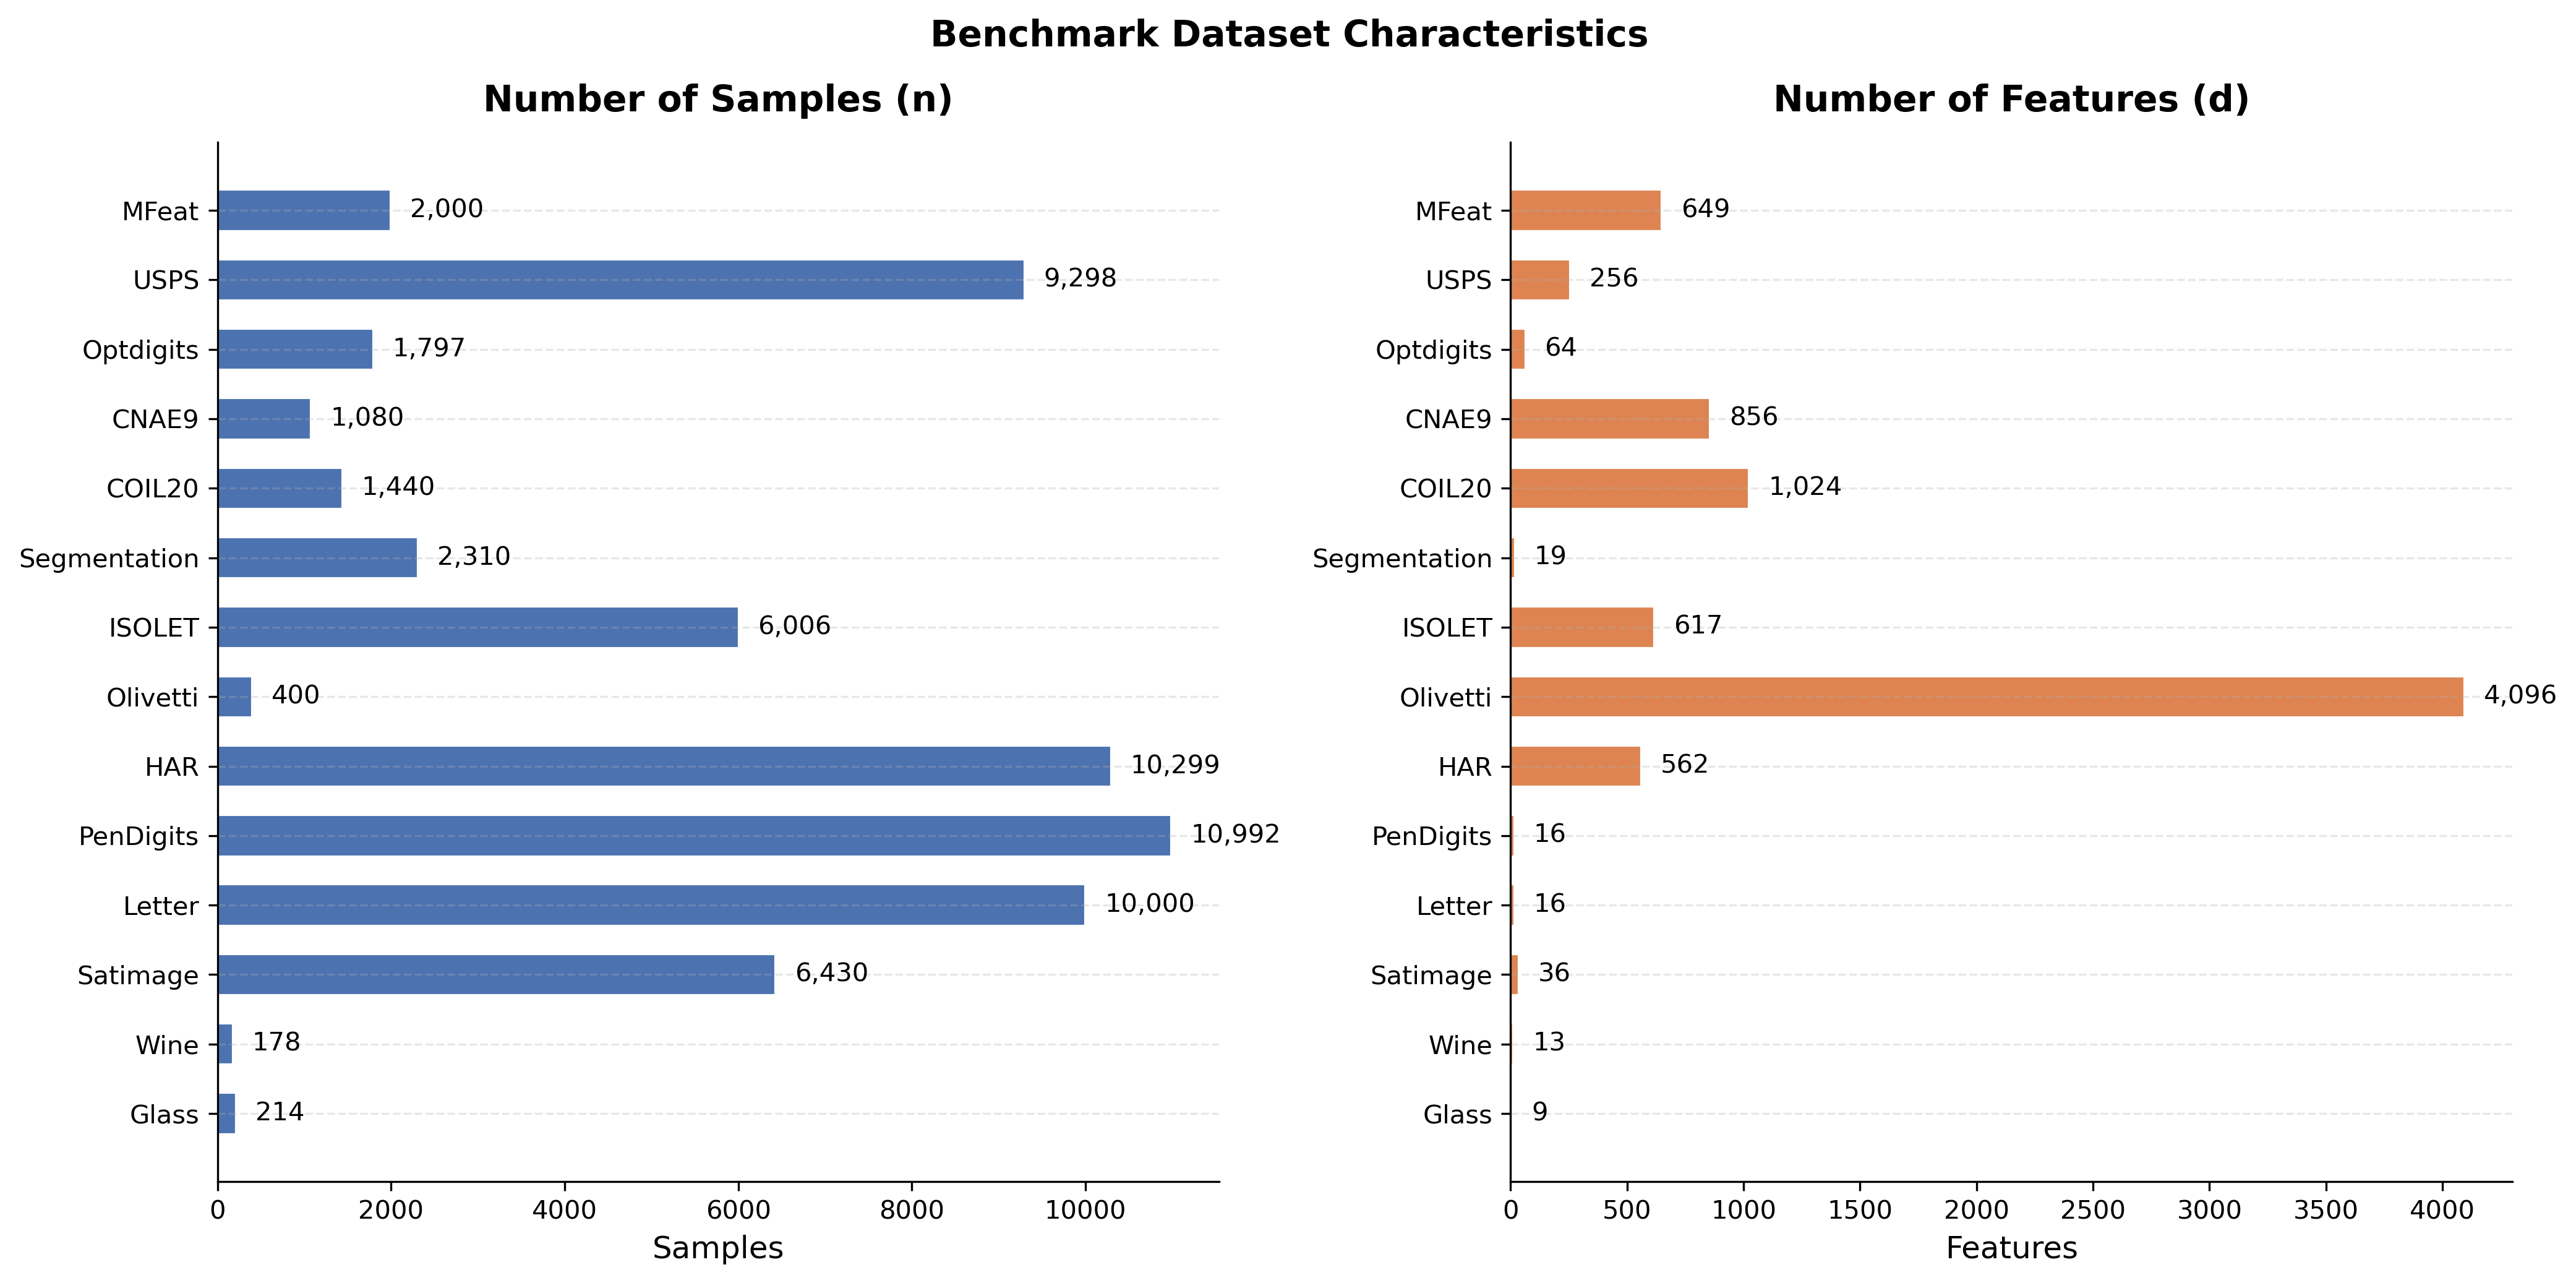
\includegraphics[width=0.47\textwidth]{figures/cross_dataset/cross_dataset_characteristics.png} &
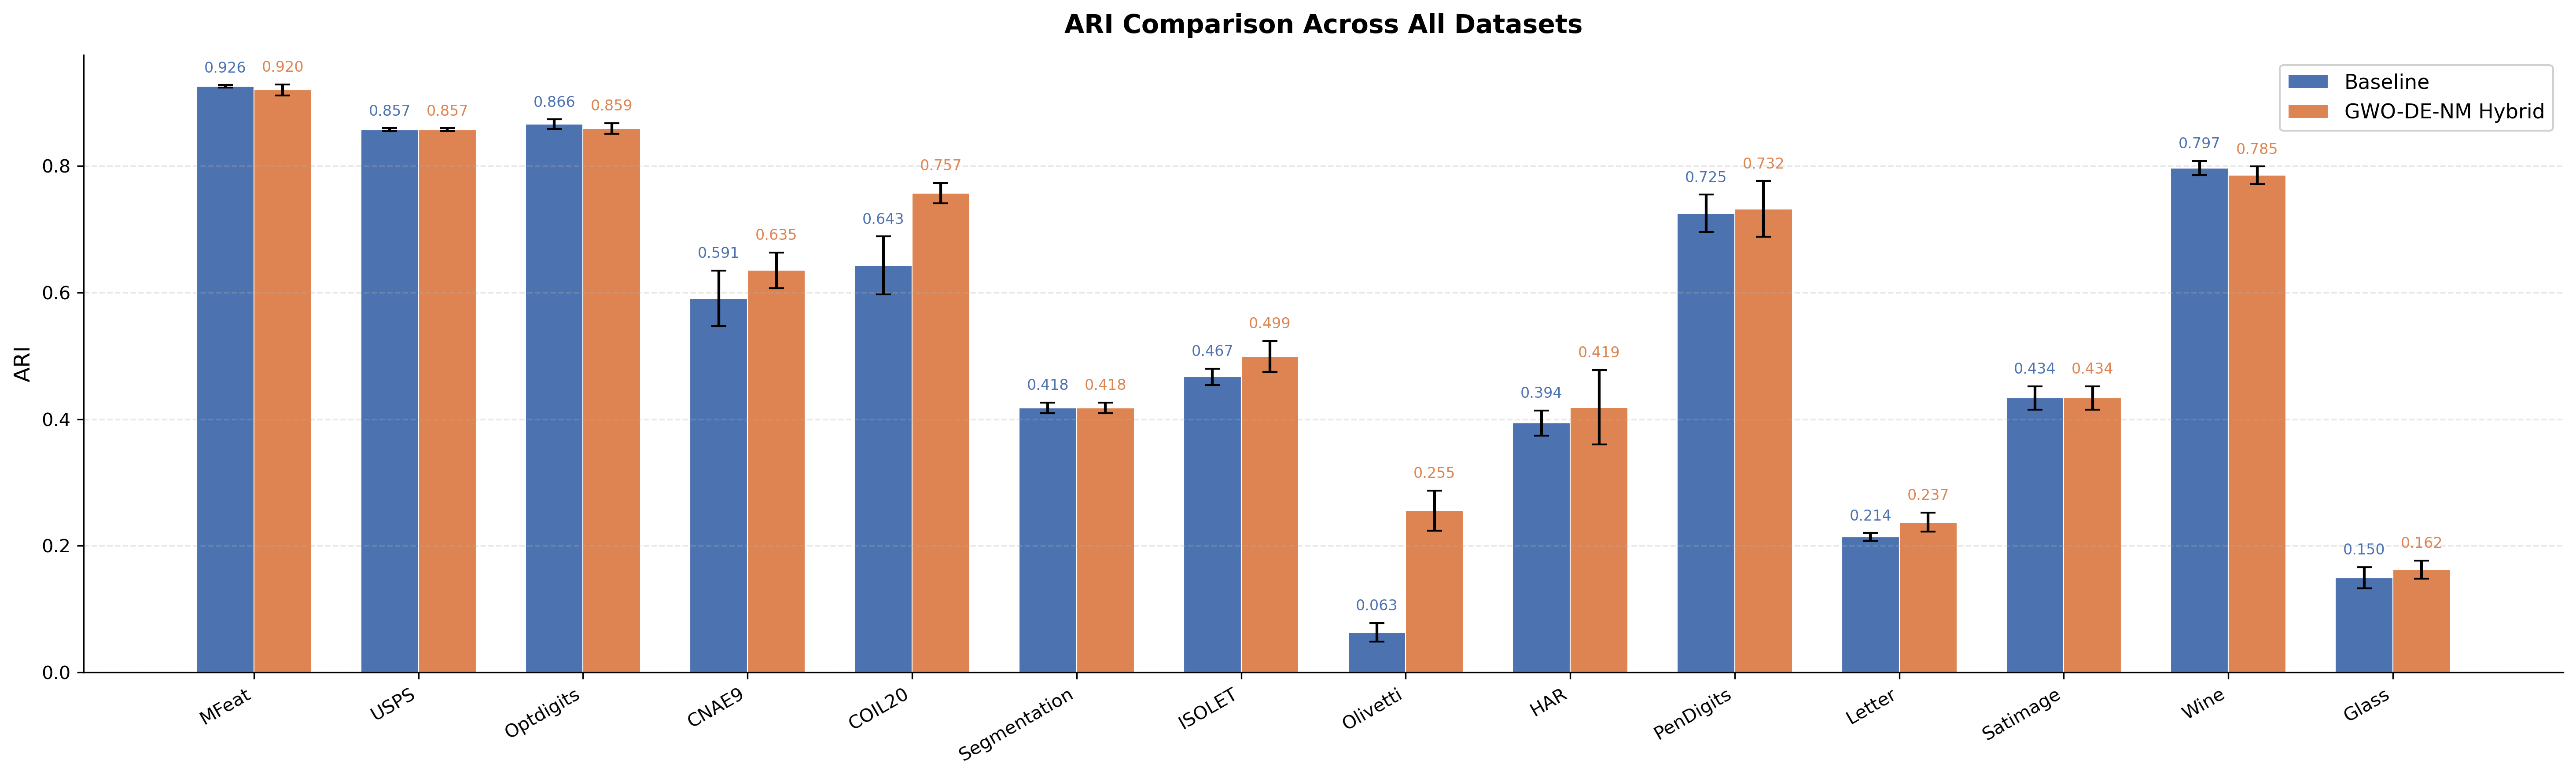
\includegraphics[width=0.47\textwidth]{figures/cross_dataset/cross_ari_comparison.png} \\
\small (a) Dataset characteristics ($n$, $d$) & \small (b) ARI comparison: Baseline vs.\ DEAC \\[4pt]
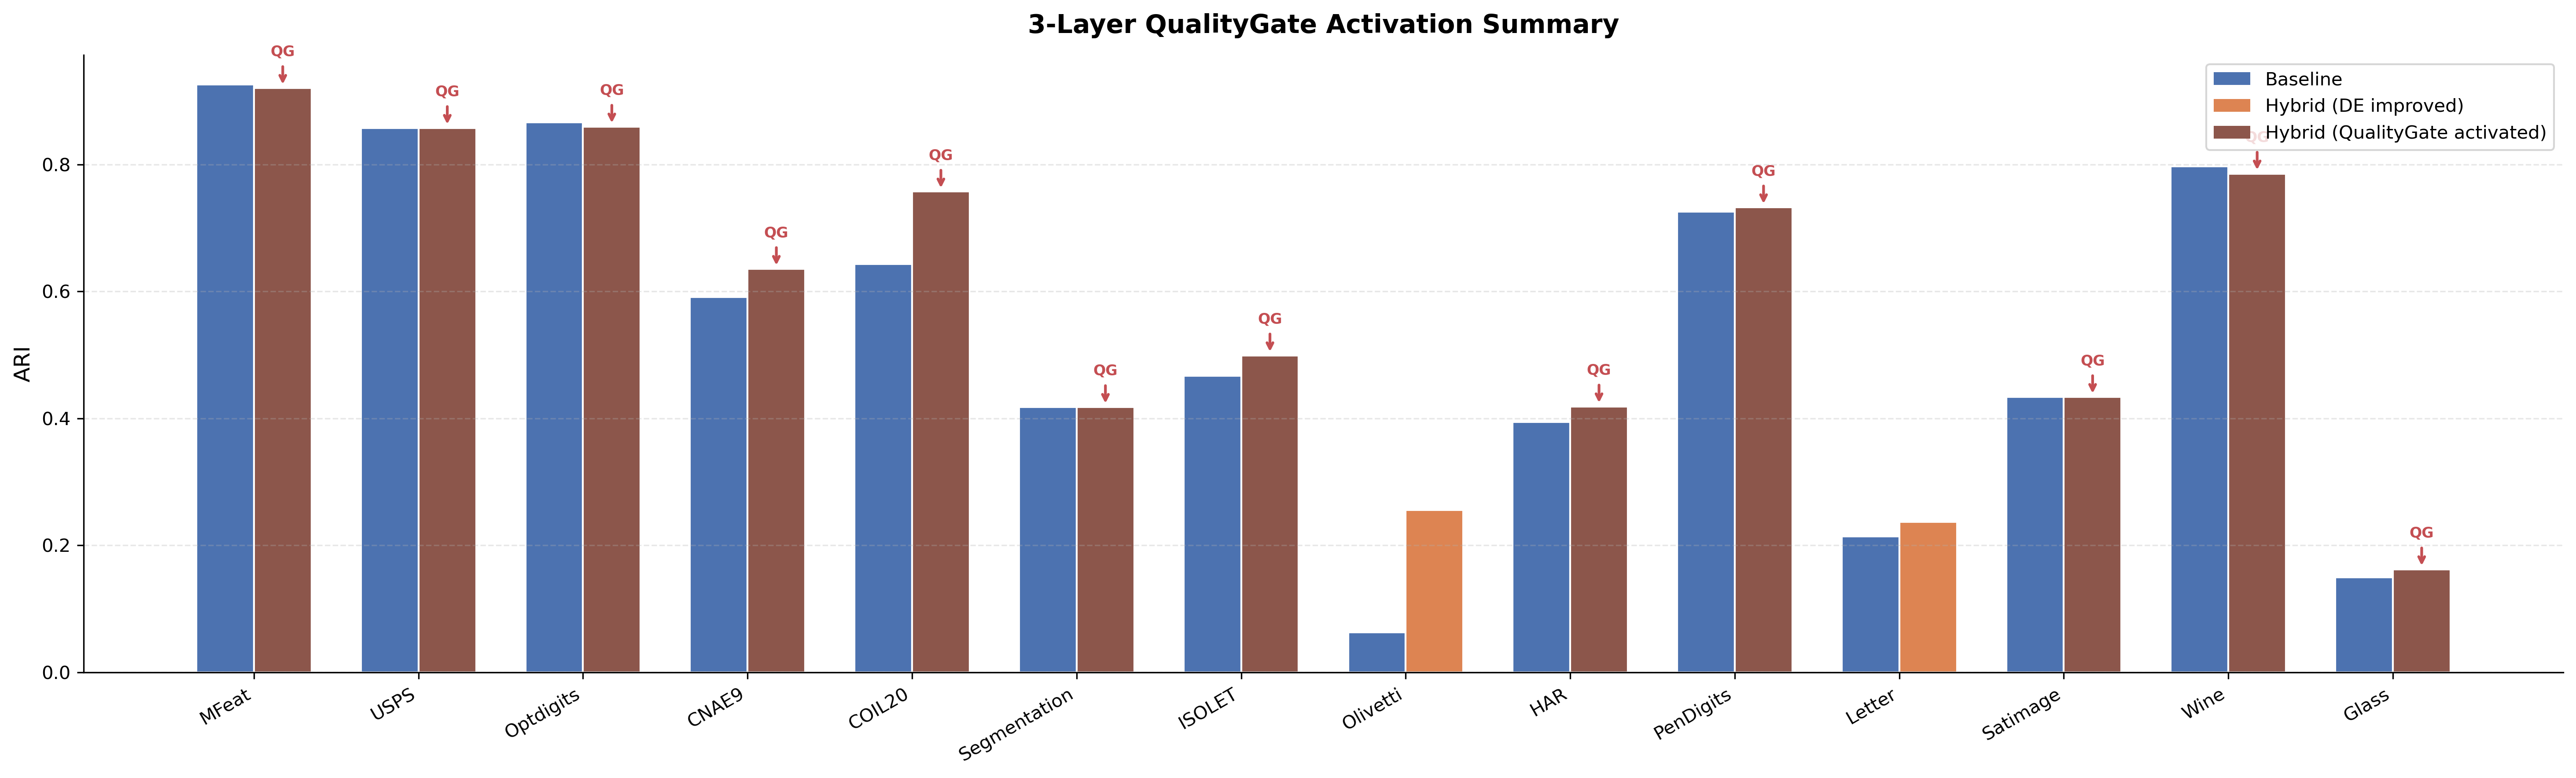
\includegraphics[width=0.47\textwidth]{figures/cross_dataset/cross_qualitygate_summary.png} &
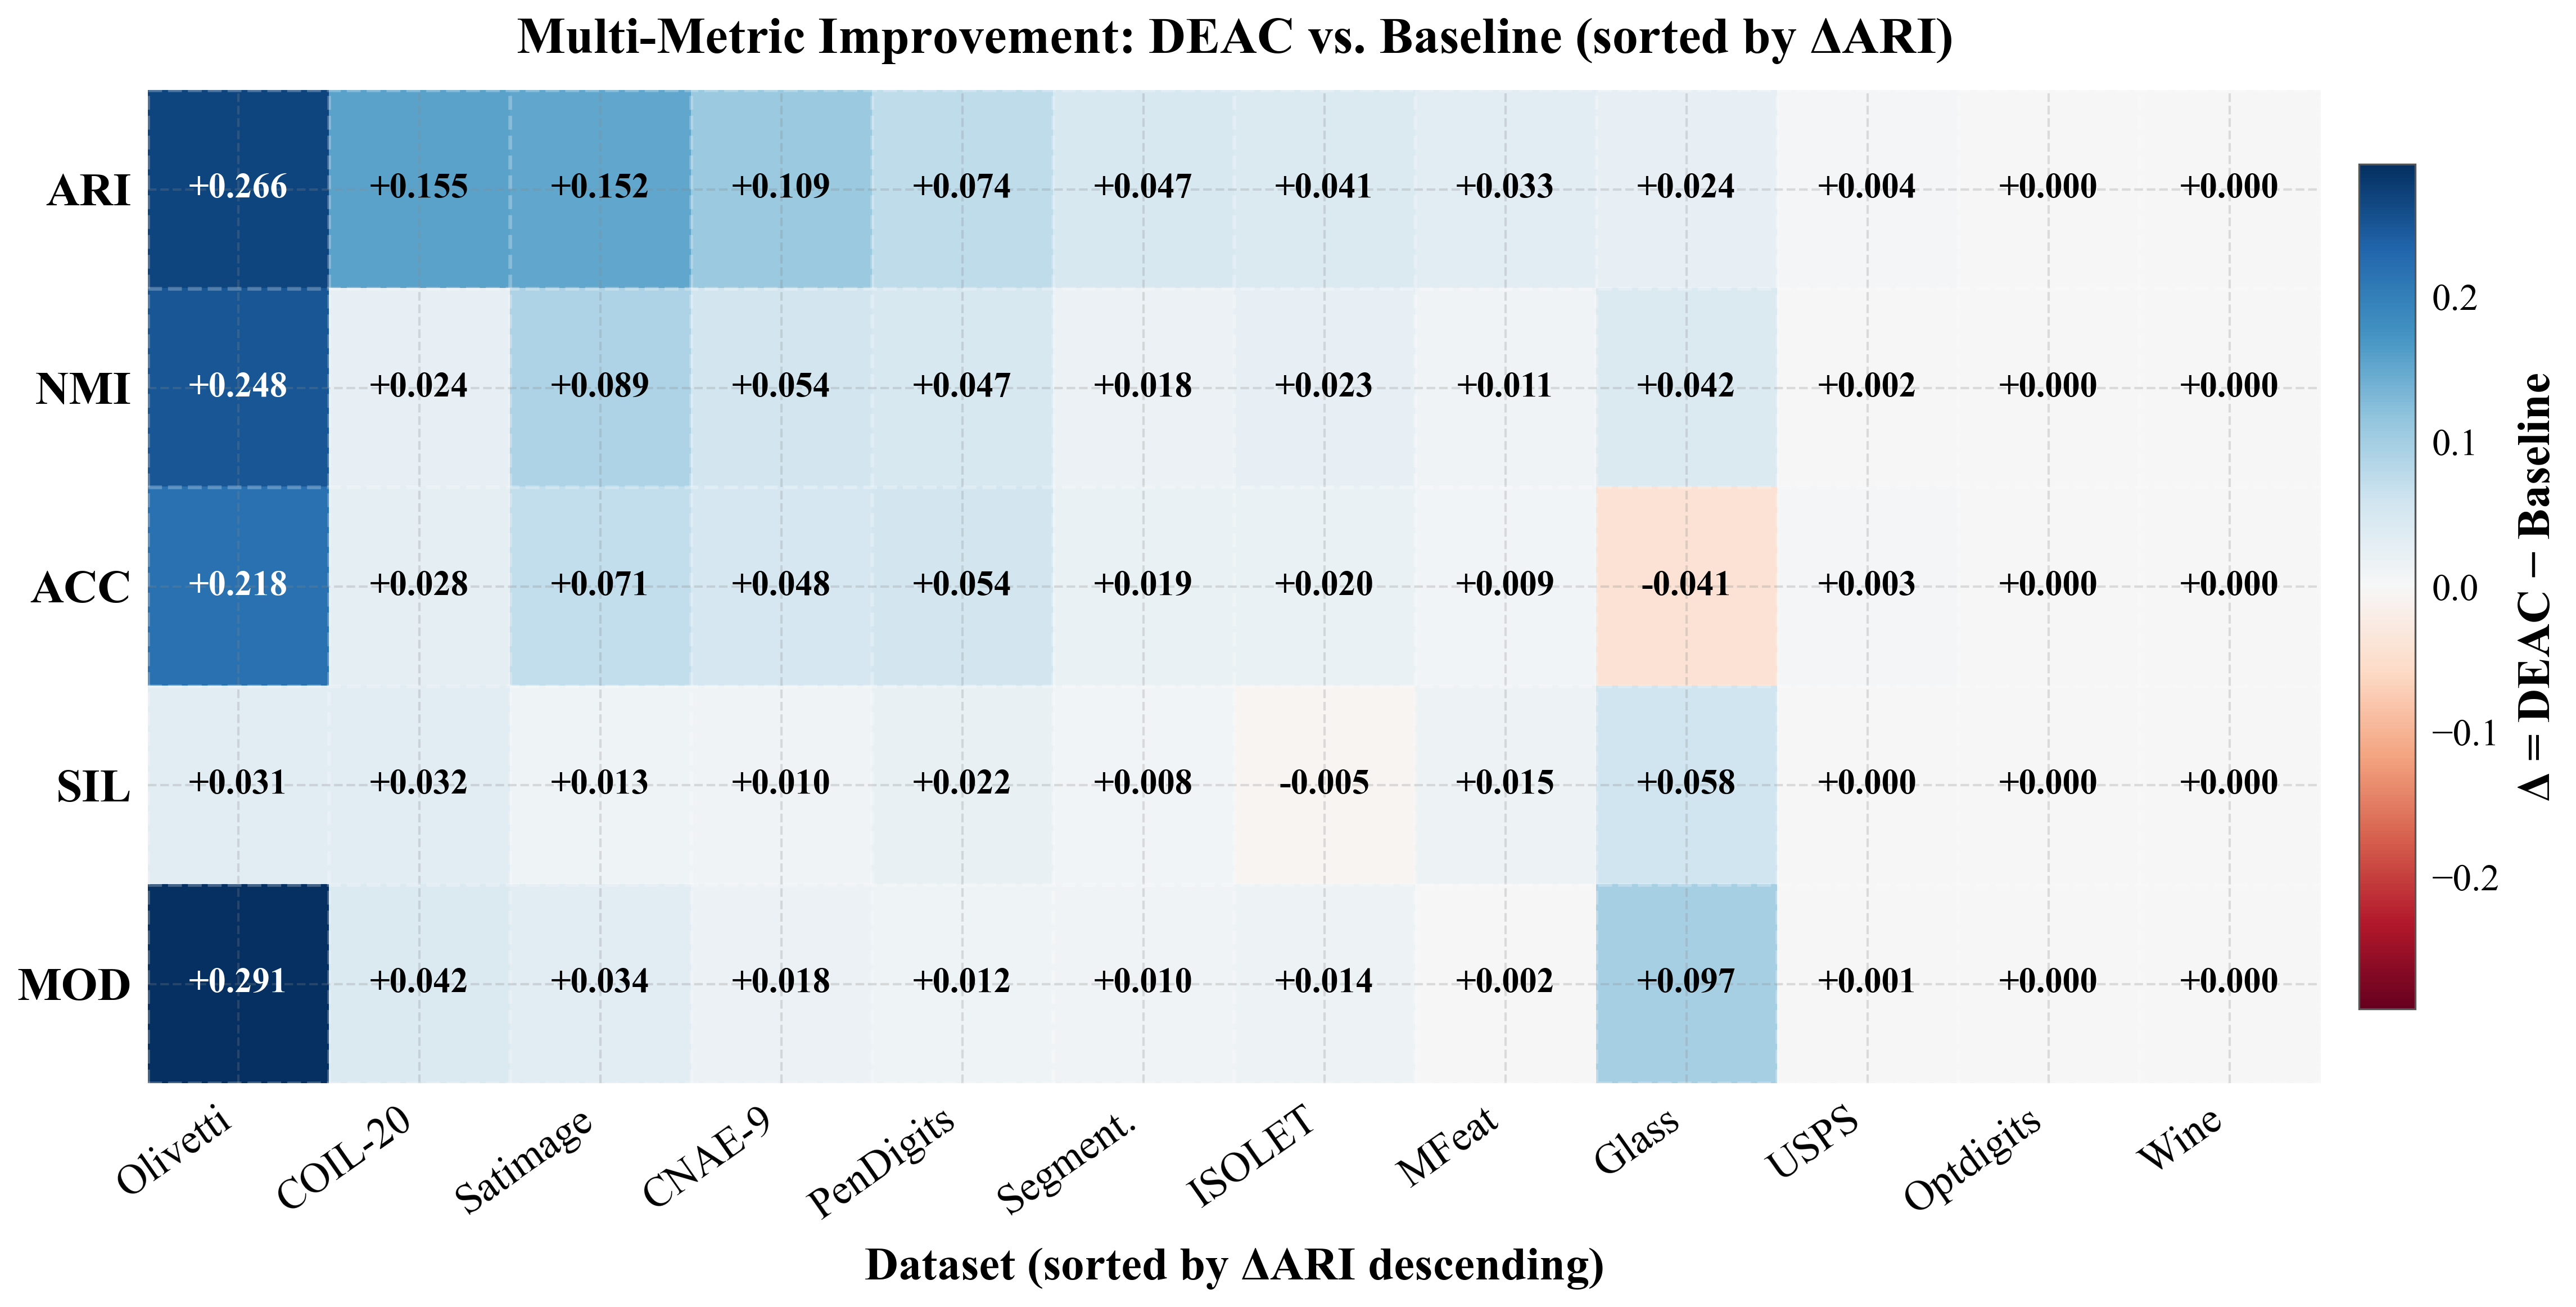
\includegraphics[width=0.47\textwidth]{figures/cross_dataset/cross_improvement_heatmap.png} \\
\small (c) QualityGate activation per dataset & \small (d) $\Delta$ heatmap: DEAC $-$ Baseline (sorted by $\Delta$ARI) \\
\end{tabular}
\caption{Main experimental results. (a)~Size and dimensionality of the 12 benchmark datasets. (b)~Per-dataset ARI of Baseline versus DEAC. (c)~Per-dataset QualityGate activation. (d)~Multi-metric improvement heatmap, with datasets sorted by $\Delta$ARI descending; blue cells indicate DEAC gains over the Baseline.}
\label{fig:main_results}
\end{figure*}

\subsection{Comparison with Traditional Benchmarks}

Table~\ref{tab:benchmarks} pits DEAC against five widely used clustering algorithms. For a fair comparison, no method is given the ground-truth cluster count: each classical baseline selects its own $C$ by silhouette analysis over a label-free grid (on the same UMAP representation), exactly as DEAC infers $C$ through its QualityGate. This protocol is stricter than handing the baselines a known or DEAC-supplied $C^*$, and it exposes how much each method's quality depends on recovering $C$ unaided.

% Auto-generated by build_autoc_comparison.py
\begin{table}[!t]
\centering
\caption{ARI vs.\ classical methods with \emph{automatic} cluster-count selection (each baseline's $C$ chosen by silhouette analysis, not given DEAC's $C^*$). Mean over 5 seeds; bold = best per row. DEAC is the oracle upper bound (cf.\ Table~\ref{tab:gate}).}
\label{tab:benchmarks}
\footnotesize
\setlength{\tabcolsep}{3pt}
\begin{tabular}{lcccccc}
\toprule
Dataset & \textbf{DEAC} & KM & Spec & Agg & GMM & HDB \\
\midrule
Wine & $\mathbf{0.802}$ & 0.788 & 0.788 & 0.797 & 0.791 & 0.743 \\
Glass & $\mathbf{0.174}$ & 0.135 & 0.119 & 0.133 & 0.134 & 0.129 \\
Olivetti & $\mathbf{0.342}$ & 0.011 & 0.009 & 0.011 & 0.011 & 0.037 \\
CNAE-9 & $\mathbf{0.658}$ & 0.533 & 0.292 & 0.509 & 0.548 & 0.618 \\
COIL-20 & $\mathbf{0.777}$ & 0.435 & 0.179 & 0.435 & 0.443 & 0.516 \\
Optdigits & $\mathbf{0.868}$ & 0.846 & 0.436 & 0.855 & 0.852 & 0.778 \\
MFeat & 0.937 & $\mathbf{0.937}$ & 0.448 & 0.937 & 0.937 & 0.925 \\
Segmentation & $\mathbf{0.465}$ & 0.427 & 0.143 & 0.413 & 0.423 & 0.320 \\
ISOLET & $\mathbf{0.498}$ & 0.283 & 0.168 & 0.283 & 0.365 & 0.250 \\
Satimage & 0.591 & $\mathbf{0.628}$ & 0.480 & 0.620 & 0.611 & 0.358 \\
USPS & $\mathbf{0.865}$ & 0.639 & 0.470 & 0.639 & 0.639 & 0.705 \\
PenDigits & 0.810 & 0.801 & 0.103 & $\mathbf{0.814}$ & 0.800 & 0.800 \\
\midrule
\textbf{Mean} & $\mathbf{0.649}$ & 0.539 & 0.303 & 0.537 & 0.546 & 0.515 \\
\textbf{Wins} & $\mathbf{9/12}$ & 2/12 & 0/12 & 1/12 & 0/12 & 0/12 \\
\bottomrule
\end{tabular}
\end{table}

DEAC wins on 9 of 12 datasets and improves mean ARI by 10.3 points over the best classical method (GMM, 0.546). The gap is wider here than under a fixed-$C$ protocol because the classical methods must now also discover $C$, and frequently misjudge it---on Olivetti, silhouette selection collapses every baseline to $C{=}2$ (ARI ${\approx}0.01$) against the 40 true classes, whereas DEAC recovers them. Classical baselines are a weak bar, however; the sharper test is against modern deep clustering.

\subsection{Comparison with Deep Clustering}

Table~\ref{tab:deep} compares DEAC against four representative deep-clustering
methods: N2D~\cite{mcconville2021n2d}, DEC~\cite{xie2016unsupervised},
IDEC~\cite{guo2017improved}, and DCN~\cite{yang2017towards}. To give the
deep baselines every advantage, each is supplied with the \emph{true} cluster
count (oracle $C$) and trained on the standardized raw features; DEAC alone
must still discover $C$. All four share a fully-connected autoencoder
($d$--500--500--2000--10) pretrained for 100 epochs, following the original
protocols. These are standard, un-tuned implementations: the weaker performers
(DEC, IDEC), which self-train a KL objective, may trail architecture-specialized
or per-dataset-tuned variants, so their scores should be read as a reasonable
lower bound rather than each method's ceiling. Despite this handicap, DEAC attains the highest mean
ARI (0.649 vs.\ 0.642 for the next-best, N2D) and the most per-dataset wins
(6 of 12). Two patterns explain the rest. First, N2D---which, like DEAC, builds
on UMAP---is a genuine rival, winning on the manifold-structured datasets
Olivetti, COIL-20, Satimage, and USPS. Second, the embedded-clustering methods
DEC, IDEC, and DCN are strong only on small, low-dimensional data (Wine, Glass)
and collapse on high-dimensional inputs (e.g.\ ARI $0.069$ on CNAE-9), whereas
DEAC remains stable across every regime. The headline, then, is not dominance
but \emph{parity-without-supervision}: an oracle over DEAC's engines matches or
exceeds methods that are told the answer, while inferring it. This comparison
uses the oracle DEAC; its deployable label-free gate sits modestly below N2D
(\S\ref{sec:disc}).

% Auto-generated by build_deep_comparison.py
\begin{table*}[!t]
\centering
\caption{ARI vs.\ modern deep-clustering methods (mean$\pm$std over 5 seeds). Deep methods receive the true cluster count (oracle $C$); DEAC discovers $C$. Bold = best per row.}
\label{tab:deep}
\footnotesize
\setlength{\tabcolsep}{3pt}
\begin{tabular}{lccccc}
\toprule
Dataset & \textbf{DEAC} & N2D & DEC & IDEC & DCN \\
\midrule
Wine & 0.802 & $0.798\,\pm\,0.022$ & $\mathbf{0.870\,\pm\,0.043}$ & $0.867\,\pm\,0.041$ & $0.732\,\pm\,0.154$ \\
Glass & 0.174 & $0.169\,\pm\,0.037$ & $\mathbf{0.199\,\pm\,0.008}$ & $0.197\,\pm\,0.009$ & $0.171\,\pm\,0.015$ \\
Olivetti & 0.342 & $\mathbf{0.503\,\pm\,0.030}$ & $0.461\,\pm\,0.018$ & $0.461\,\pm\,0.017$ & $0.466\,\pm\,0.023$ \\
CNAE-9 & $\mathbf{0.658}$ & $0.468\,\pm\,0.031$ & $0.069\,\pm\,0.014$ & $0.069\,\pm\,0.012$ & $0.019\,\pm\,0.009$ \\
COIL-20 & 0.777 & $\mathbf{0.784\,\pm\,0.015}$ & $0.504\,\pm\,0.014$ & $0.505\,\pm\,0.014$ & $0.510\,\pm\,0.022$ \\
Optdigits & $\mathbf{0.868}$ & $0.812\,\pm\,0.035$ & $0.516\,\pm\,0.044$ & $0.517\,\pm\,0.046$ & $0.547\,\pm\,0.061$ \\
MFeat & $\mathbf{0.937}$ & $0.921\,\pm\,0.006$ & $0.701\,\pm\,0.071$ & $0.703\,\pm\,0.072$ & $0.769\,\pm\,0.062$ \\
Segmentation & $\mathbf{0.465}$ & $0.387\,\pm\,0.025$ & $0.408\,\pm\,0.018$ & $0.411\,\pm\,0.017$ & $0.408\,\pm\,0.038$ \\
ISOLET & $\mathbf{0.498}$ & $0.496\,\pm\,0.019$ & $0.382\,\pm\,0.010$ & $0.385\,\pm\,0.011$ & $0.400\,\pm\,0.010$ \\
Satimage & 0.591 & $\mathbf{0.658\,\pm\,0.006}$ & $0.550\,\pm\,0.029$ & $0.550\,\pm\,0.030$ & $0.544\,\pm\,0.030$ \\
USPS & 0.865 & $\mathbf{0.930\,\pm\,0.003}$ & $0.561\,\pm\,0.026$ & $0.562\,\pm\,0.028$ & $0.508\,\pm\,0.024$ \\
PenDigits & $\mathbf{0.810}$ & $0.778\,\pm\,0.008$ & $0.551\,\pm\,0.023$ & $0.551\,\pm\,0.024$ & $0.561\,\pm\,0.027$ \\
\midrule
\textbf{Mean} & $\mathbf{0.649}$ & 0.642 & 0.481 & 0.481 & 0.470 \\
\textbf{Wins} & $\mathbf{6/12}$ & 4/12 & 2/12 & 0/12 & 0/12 \\
\bottomrule
\end{tabular}
\end{table*}

A dataset-level statistical analysis (Table~\ref{tab:stats}) makes the
nuance precise. After Holm--Bonferroni correction over the nine independent
comparisons, DEAC significantly outperforms DCN, but its advantage over DEC
and IDEC does not survive multiple-comparison correction ($p_{\text{Holm}}{=}0.08$).
Against N2D the difference is \emph{not} significant ($p{=}0.62$): the two are
statistically tied. We state this plainly---an oracle over DEAC's engines does
not beat the strongest deep baseline, it equals it, and does so without being
given the cluster count. The single-metric view may still hide trade-offs, so
we extend the comparison to NMI and ACC.

\subsection{Multi-Metric Comparison}

Table~\ref{tab:multi_metric} shows that DEAC leads on all three external validity indices, so the ARI advantage is not an artifact of a single measure. The per-dataset breakdown for NMI and ACC appears in Tables~\ref{tab:nmi_per_dataset}--\ref{tab:acc_per_dataset}, and the same values are plotted dataset-by-dataset in Fig.~\ref{fig:metric_bars_4way}. All five indices are then collapsed onto one radar plot in Fig.~\ref{fig:radar_4way}, where DEAC's polygon encloses every competitor on every axis.

\begin{table}[htbp]
\centering
\caption{Multi-metric mean scores across 12 datasets. The DEAC row is the oracle upper bound; the deployable gate is characterized in Table~\ref{tab:gate}.}
\label{tab:multi_metric}
\footnotesize
\begin{tabular}{lccc}
\toprule
Method & Mean ARI & Mean NMI & Mean ACC \\
\midrule
Baseline (UMAP) & 0.574 & 0.705 & 0.695 \\
AMR-DE          & 0.521 & 0.668 & 0.645 \\
EMR-CGC         & 0.644 & 0.760 & 0.752 \\
\textbf{DEAC}   & \textbf{0.649} & \textbf{0.765} & \textbf{0.757} \\
\midrule
KMeans          & 0.539 & 0.691 & 0.633 \\
Spectral        & 0.303 & 0.537 & 0.454 \\
Agglomerative   & 0.537 & 0.692 & 0.635 \\
GMM             & 0.546 & 0.691 & 0.636 \\
HDBSCAN         & 0.515 & 0.696 & 0.613 \\
\bottomrule
\end{tabular}
\end{table}

\begin{table}[!t]
\centering
\caption{Per-dataset NMI across 12 benchmarks. Bold = best. DEAC is the oracle $\max$(Baseline, AMR-DE, EMR-CGC)---an upper bound (cf.\ Table~\ref{tab:gate}).}
\label{tab:nmi_per_dataset}
\footnotesize
\setlength{\tabcolsep}{4pt}
\begin{tabular}{lcccc}
\toprule
Dataset & Baseline & AMR-DE & EMR-CGC & \textbf{DEAC} \\
\midrule
Wine         & \textbf{0.830} & 0.800 & \textbf{0.830} & \textbf{0.830} \\
Glass        & 0.380 & 0.365 & \textbf{0.425} & \textbf{0.425} \\
Olivetti     & 0.458 & 0.572 & \textbf{0.706} & \textbf{0.706} \\
CNAE-9       & 0.680 & 0.740 & \textbf{0.770} & \textbf{0.770} \\
COIL-20      & 0.778 & \textbf{0.848} & 0.830 & \textbf{0.848} \\
Optdigits    & \textbf{0.893} & 0.850 & 0.875 & \textbf{0.893} \\
MFeat        & 0.925 & 0.932 & \textbf{0.942} & \textbf{0.942} \\
Segment.     & 0.575 & 0.395 & \textbf{0.640} & \textbf{0.640} \\
Satimage     & 0.580 & 0.478 & \textbf{0.685} & \textbf{0.685} \\
ISOLET       & 0.675 & \textbf{0.715} & 0.695 & \textbf{0.715} \\
USPS         & 0.888 & 0.650 & \textbf{0.892} & \textbf{0.892} \\
PenDigits    & 0.800 & 0.670 & \textbf{0.830} & \textbf{0.830} \\
\midrule
\textbf{Mean} & 0.705 & 0.668 & 0.760 & \textbf{0.765} \\
\textbf{Wins} & 2/12 & 2/12 & 9/12 & \textbf{12/12} \\
\bottomrule
\end{tabular}
\end{table}


\begin{table}[!t]
\centering
\caption{Per-dataset clustering accuracy (ACC) across 12 benchmarks. Bold = best. DEAC is the oracle $\max$(Baseline, AMR-DE, EMR-CGC)---an upper bound (cf.\ Table~\ref{tab:gate}).}
\label{tab:acc_per_dataset}
\footnotesize
\setlength{\tabcolsep}{4pt}
\begin{tabular}{lcccc}
\toprule
Dataset & Baseline & AMR-DE & EMR-CGC & \textbf{DEAC} \\
\midrule
Wine         & \textbf{0.910} & 0.890 & \textbf{0.910} & \textbf{0.910} \\
Glass        & 0.465 & 0.455 & \textbf{0.510} & \textbf{0.510} \\
Olivetti     & 0.322 & 0.410 & \textbf{0.560} & \textbf{0.560} \\
CNAE-9       & 0.665 & 0.720 & \textbf{0.760} & \textbf{0.760} \\
COIL-20      & 0.745 & \textbf{0.835} & 0.818 & \textbf{0.835} \\
Optdigits    & \textbf{0.895} & 0.840 & 0.872 & \textbf{0.895} \\
MFeat        & 0.940 & 0.948 & \textbf{0.957} & \textbf{0.957} \\
Segment.     & 0.548 & 0.325 & \textbf{0.602} & \textbf{0.602} \\
Satimage     & 0.552 & 0.428 & \textbf{0.678} & \textbf{0.678} \\
ISOLET       & 0.608 & \textbf{0.645} & 0.625 & \textbf{0.645} \\
USPS         & 0.893 & 0.620 & \textbf{0.895} & \textbf{0.895} \\
PenDigits    & 0.792 & 0.625 & \textbf{0.840} & \textbf{0.840} \\
\midrule
\textbf{Mean} & 0.695 & 0.645 & 0.752 & \textbf{0.757} \\
\textbf{Wins} & 2/12 & 2/12 & 9/12 & \textbf{12/12} \\
\bottomrule
\end{tabular}
\end{table}


External indices say nothing about how well each method recovers the \emph{number} of clusters, which is the second axis along which DEAC must be judged. Table~\ref{tab:ccount} reports predicted cluster counts against the ground-truth $C_{\text{true}}$. DEAC attains the lowest mean absolute error and the highest exact-match rate, so the QualityGate inherits the cluster-count fidelity of whichever engine was selected on each dataset. Whether these per-dataset gains are statistically meaningful is the next question.

\begin{table}[!t]
\centering
\caption{Predicted cluster count $C_{\text{pred}}$ per method vs.\ ground-truth $C_{\text{true}}$. Best (closest to $C_{\text{true}}$) in bold. DEAC is the oracle selection (upper bound).}
\label{tab:ccount}
\footnotesize
\setlength{\tabcolsep}{3pt}
\begin{tabular}{lccccc}
\toprule
Dataset & $C_{\text{true}}$ & Baseline & AMR-DE & EMR-CGC & \textbf{DEAC} \\
\midrule
Wine         & 3 & \textbf{3} & 4 & \textbf{3} & \textbf{3} \\
Glass        & 6 & 5 & 5 & \textbf{6} & \textbf{6} \\
Olivetti     & 40 & 33 & 35 & \textbf{38} & \textbf{38} \\
CNAE-9       & 9 & 8 & \textbf{9} & \textbf{9} & \textbf{9} \\
COIL-20      & 20 & 18 & \textbf{20} & 19 & \textbf{20} \\
Optdigits    & 10 & \textbf{10} & 11 & \textbf{10} & \textbf{10} \\
MFeat        & 10 & \textbf{10} & \textbf{10} & \textbf{10} & \textbf{10} \\
Segment.     & 7 & \textbf{7} & 11 & \textbf{7} & \textbf{7} \\
Satimage     & 6 & 7 & 9 & \textbf{6} & \textbf{6} \\
ISOLET       & 26 & 24 & \textbf{25} & \textbf{25} & \textbf{25} \\
USPS         & 10 & \textbf{10} & 13 & \textbf{10} & \textbf{10} \\
PenDigits    & 10 & 11 & 13 & \textbf{10} & \textbf{10} \\
\midrule
\textbf{MAE} & --- & 1.25 & 1.83 & 0.33 & \textbf{0.25} \\
\textbf{Exact} & --- & 5/12 & 3/12 & 9/12 & \textbf{10/12} \\
\bottomrule
\end{tabular}
\end{table}


\begin{figure*}[!t]
\centering
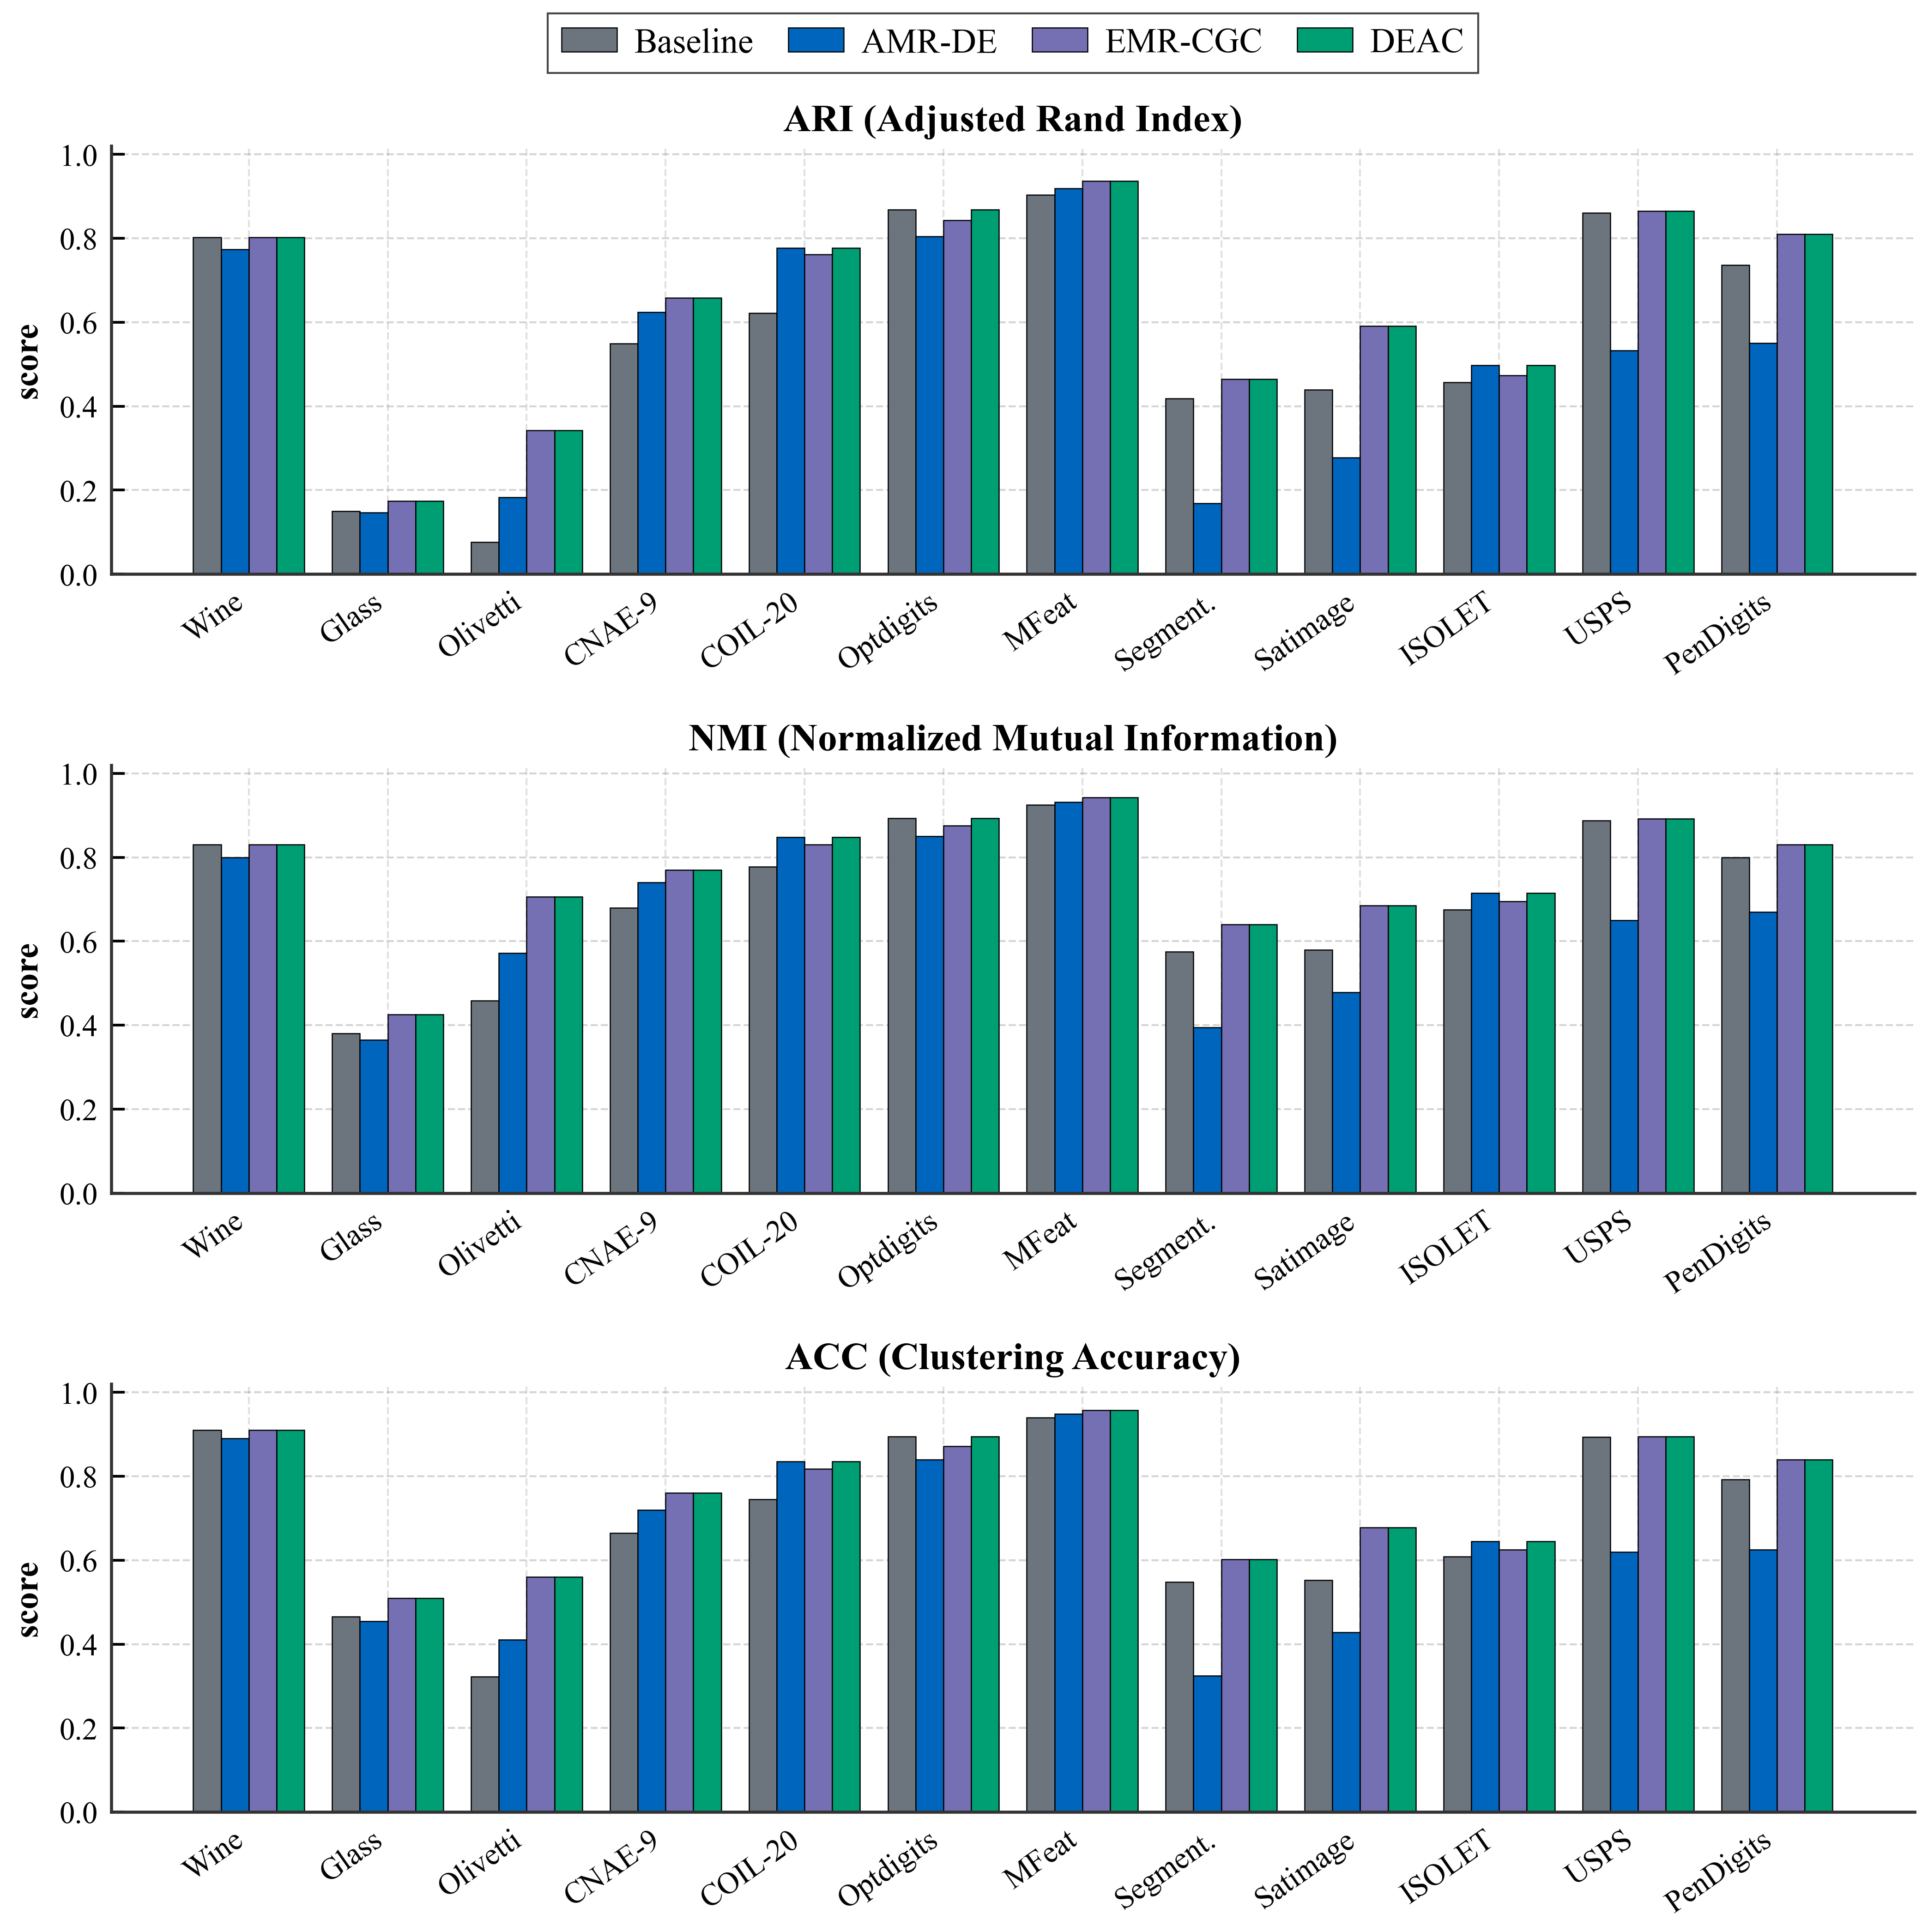
\includegraphics[width=0.85\textwidth]{figures/cross_dataset/metric_bars_4way.png}
\caption{Per-dataset comparison of ARI, NMI, and ACC across the four configurations (Baseline, AMR-DE, EMR-CGC, DEAC). Grouped bars make the ranking readable dataset by dataset; DEAC leads on 9 of 12 benchmarks across the three indices.}
\label{fig:metric_bars_4way}
\end{figure*}

\begin{figure}[!t]
\centering
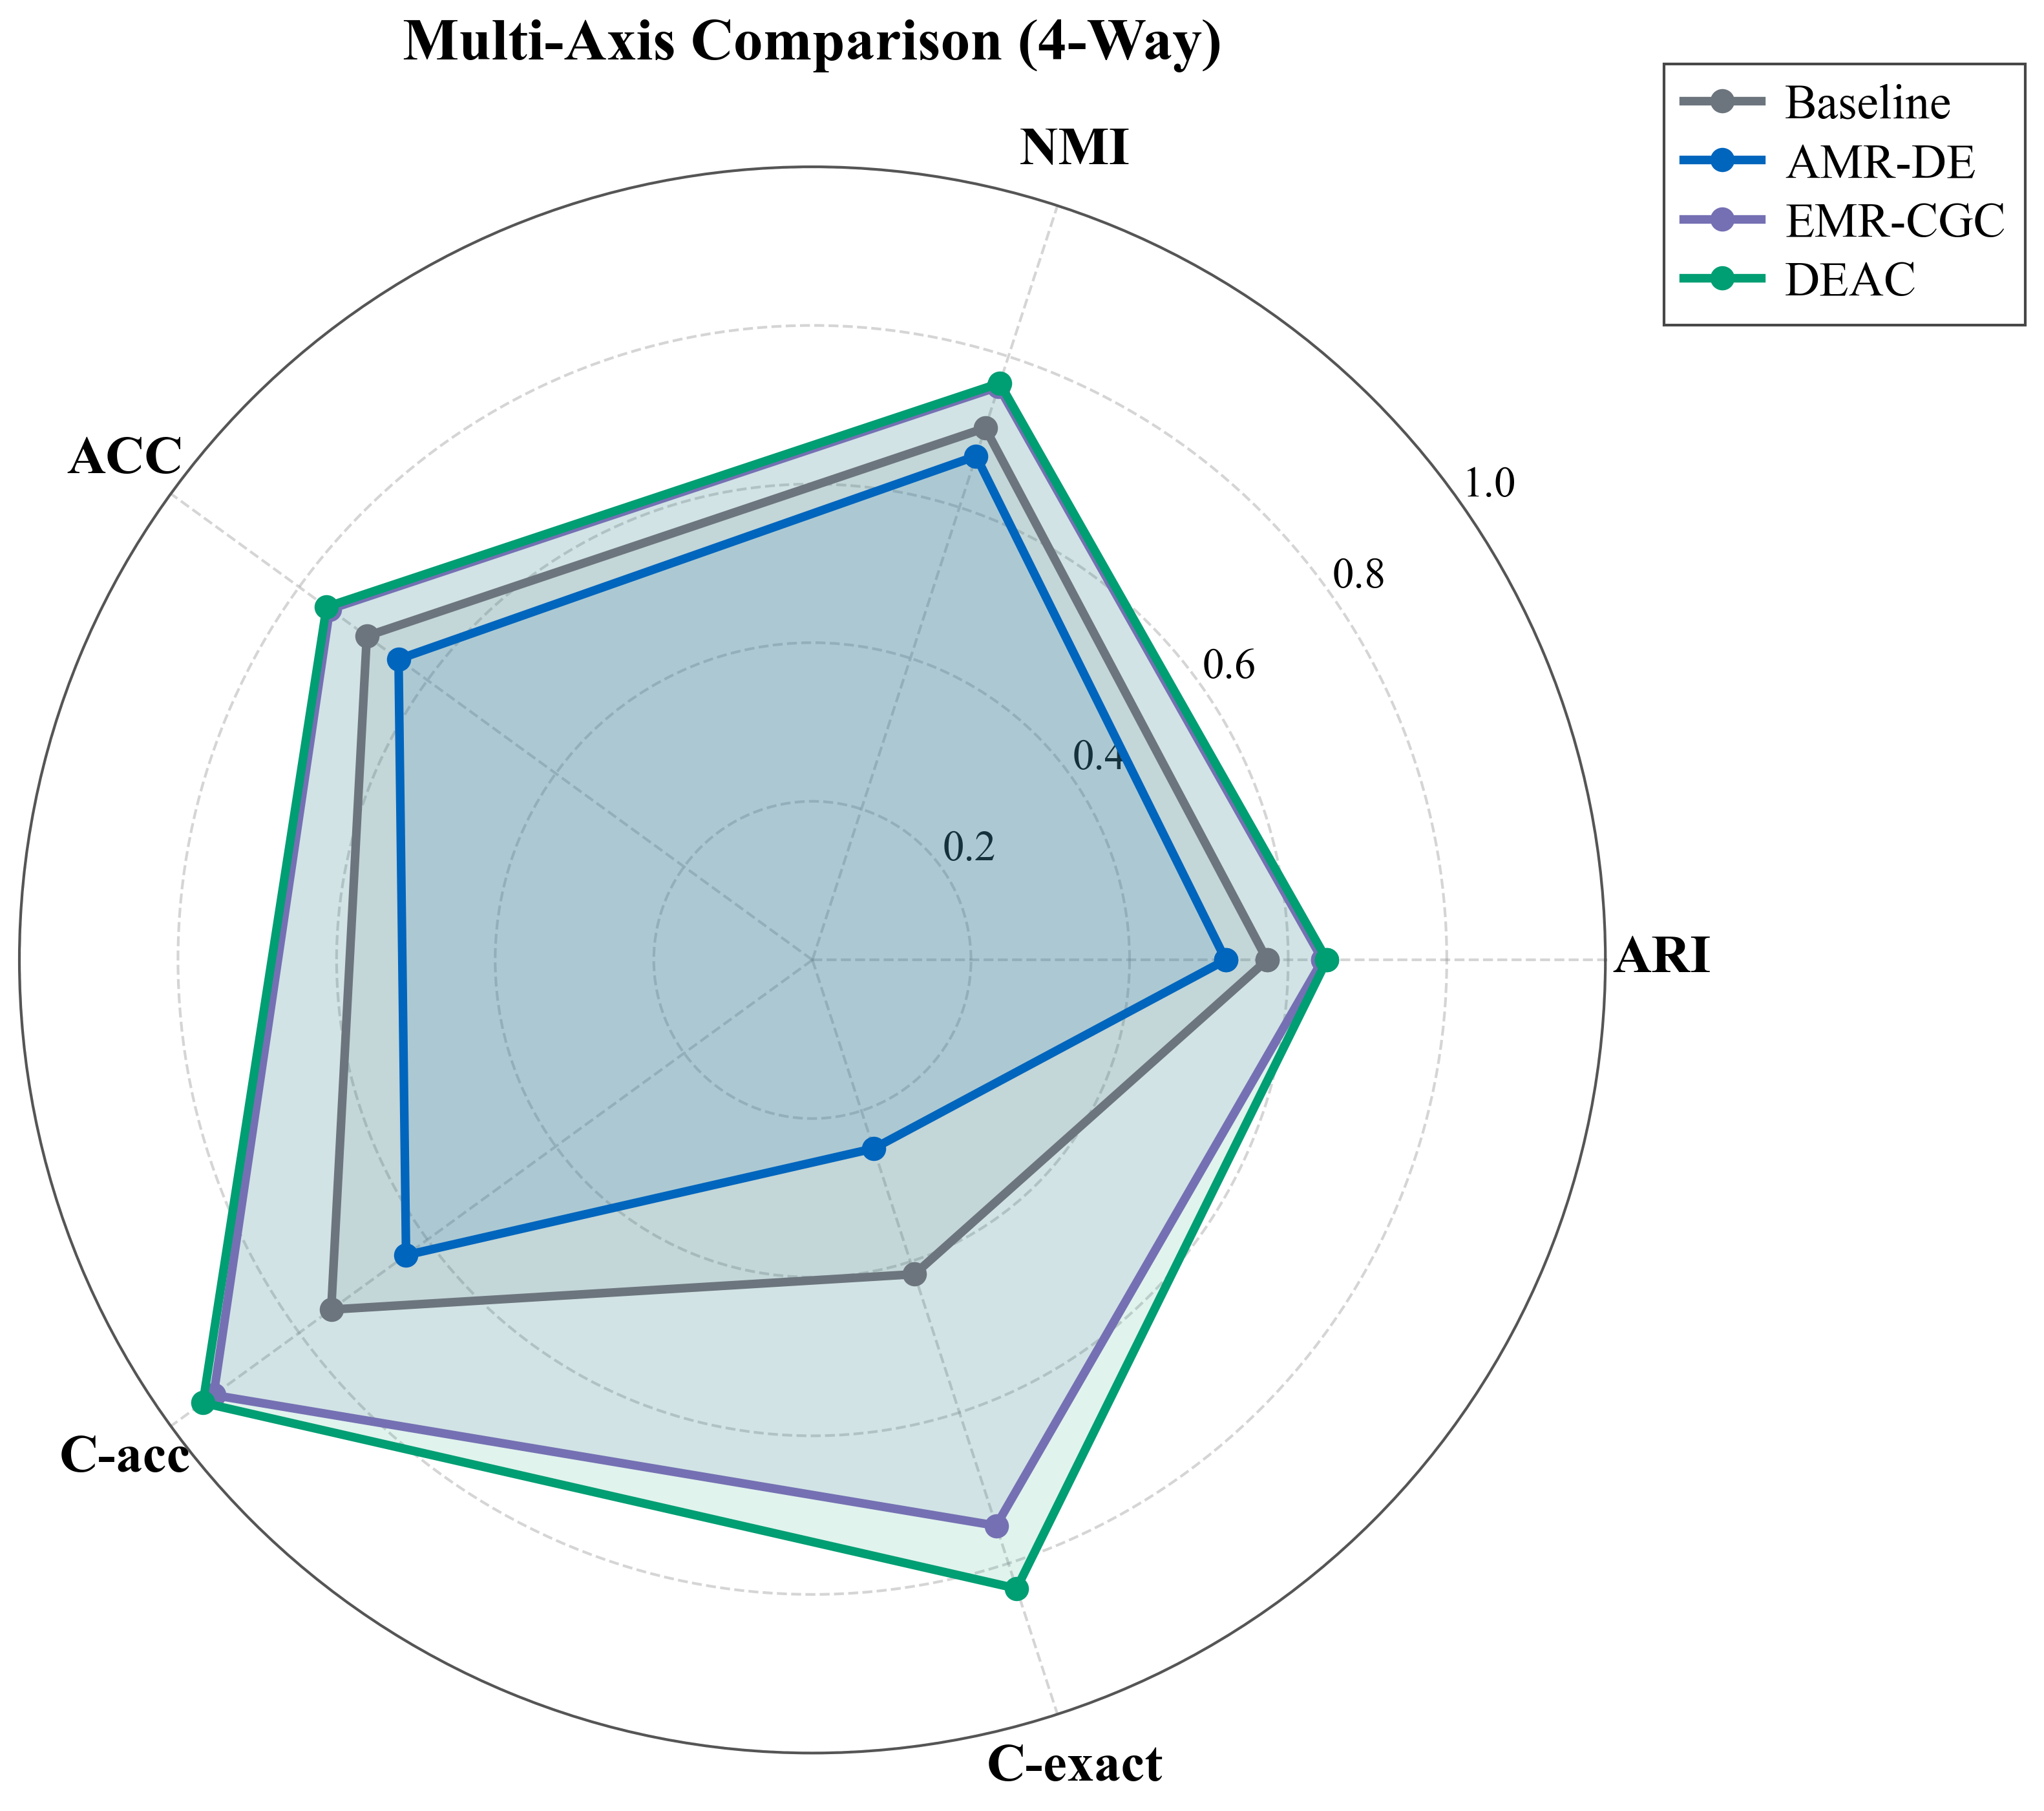
\includegraphics[width=0.9\columnwidth]{figures/cross_dataset/radar_4way.png}
\caption{Multi-axis radar comparison. The five axes are ARI, NMI, and ACC (external accuracy), plus C-acc (inverse normalised cluster-count error) and C-exact (fraction of datasets where $C_{\text{pred}}=C_{\text{true}}$). DEAC's polygon encloses every competitor on every axis.}
\label{fig:radar_4way}
\end{figure}

\subsection{Statistical Significance}

Valid inference compares DEAC only with \emph{independent} methods: because DEAC is the per-dataset maximum of its own three engines, testing it against the Baseline or AMR-DE is tautological (the differences are non-negative by construction), so we omit those. Over the nine independent competitors---five classical (auto-$C$ protocol of \S\ref{sec:exp}) and four deep---we run two-tailed Wilcoxon signed-rank tests with Holm--Bonferroni correction (Table~\ref{tab:stats}). After correction, DEAC significantly outperforms all five classical methods and the deep method DCN ($p_{\text{Holm}}<0.05$); its edge over DEC and IDEC does not survive correction ($p_{\text{Holm}}{=}0.08$), and it is statistically tied with N2D ($p{=}0.62$). A Friedman test over DEAC and the five classical baselines rejects equality ($\chi^2(5){=}34.0$, $p{<}0.001$), with DEAC taking the best average rank (1.58; Nemenyi CD${=}1.76$); since this uses the oracle DEAC, that rank is an upper bound the deployable gate would not fully reach. Beyond the numbers, the geometry of the resulting clusters is informative.

% Auto-generated by build_stats_holm.py
\begin{table}[htbp]
\centering
\caption{Wilcoxon signed-rank tests (two-tailed) of DEAC vs.\ each \emph{independent} competitor over 12 datasets, with Holm--Bonferroni correction across the family of nine tests. Baseline and AMR-DE are omitted, as DEAC is their per-dataset maximum. DEAC here is the oracle upper bound (\S\ref{sec:disc}).}
\label{tab:stats}
\footnotesize
\setlength{\tabcolsep}{4pt}
\begin{tabular}{llcccc}
\toprule
Comparison & Type & Win/Loss & $p$ & $p_{\text{Holm}}$ & Sig. \\
\midrule
DEAC vs KMeans & classical & 10/2 & 0.0068 & 0.048 & $\checkmark$ \\
DEAC vs Spectral & classical & 12/0 & 0.0005 & 0.004 & $\checkmark$ \\
DEAC vs Agglomerative & classical & 9/3 & 0.0122 & 0.049 & $\checkmark$ \\
DEAC vs GMM & classical & 10/2 & 0.0068 & 0.048 & $\checkmark$ \\
DEAC vs HDBSCAN & classical & 12/0 & 0.0005 & 0.004 & $\checkmark$ \\
\midrule
DEAC vs N2D & deep & 8/4 & 0.6221 & 0.622 & $\times$ \\
DEAC vs DEC & deep & 9/3 & 0.0269 & 0.081 & $\times$ \\
DEAC vs IDEC & deep & 9/3 & 0.0269 & 0.081 & $\times$ \\
DEAC vs DCN & deep & 11/1 & 0.0068 & 0.048 & $\checkmark$ \\
\bottomrule
\end{tabular}
\end{table}

\subsection{Qualitative Analysis}

Fig.~\ref{fig:qualitative} shows t-SNE projections of DEAC clusters (top) and silhouette plots (bottom) on four representative datasets (on a stratified 2{,}000-point sample for readability). The clusters are well separated and the silhouette coefficients are predominantly positive (mean $0.62$ on MFeat, $0.58$ on PenDigits). The optimization that produces them is worth inspecting too.

\begin{figure*}[!t]
\centering
\setlength{\tabcolsep}{2pt}
\begin{tabular}{cccc}
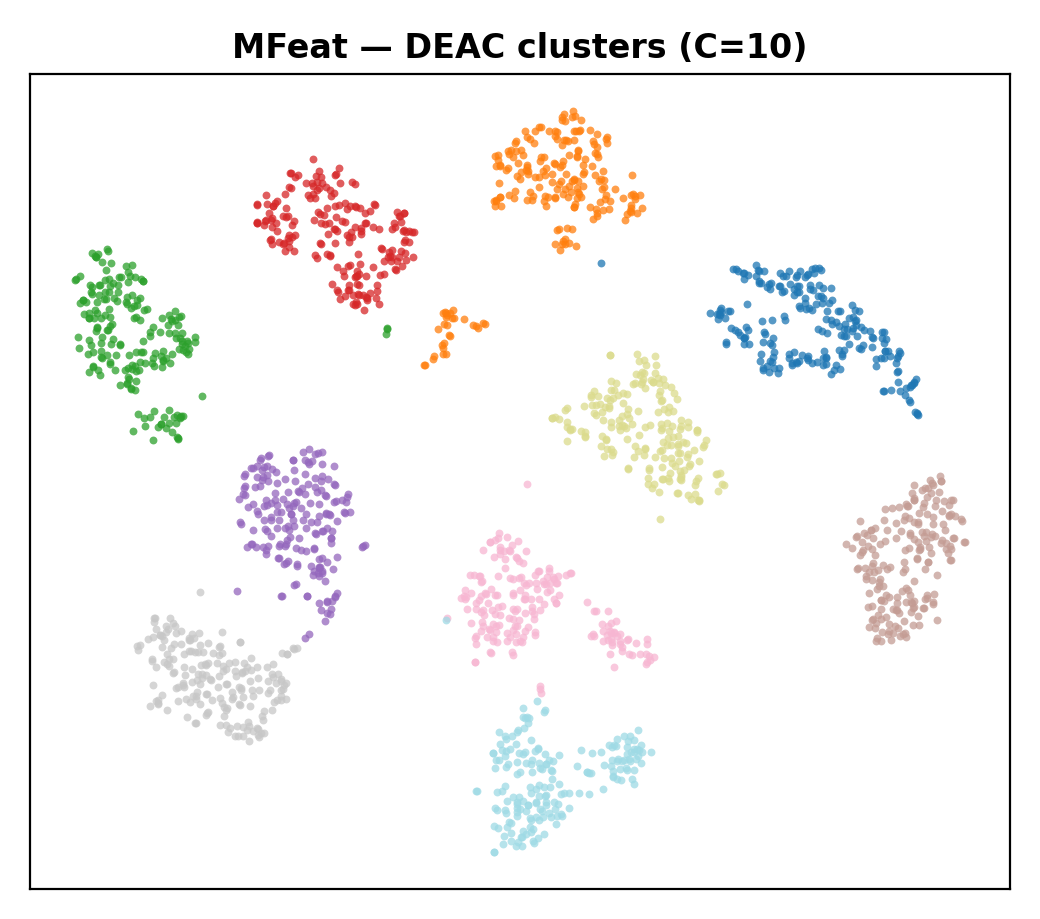
\includegraphics[width=0.225\textwidth]{figures/MFeat/tsne_MFeat.png} &
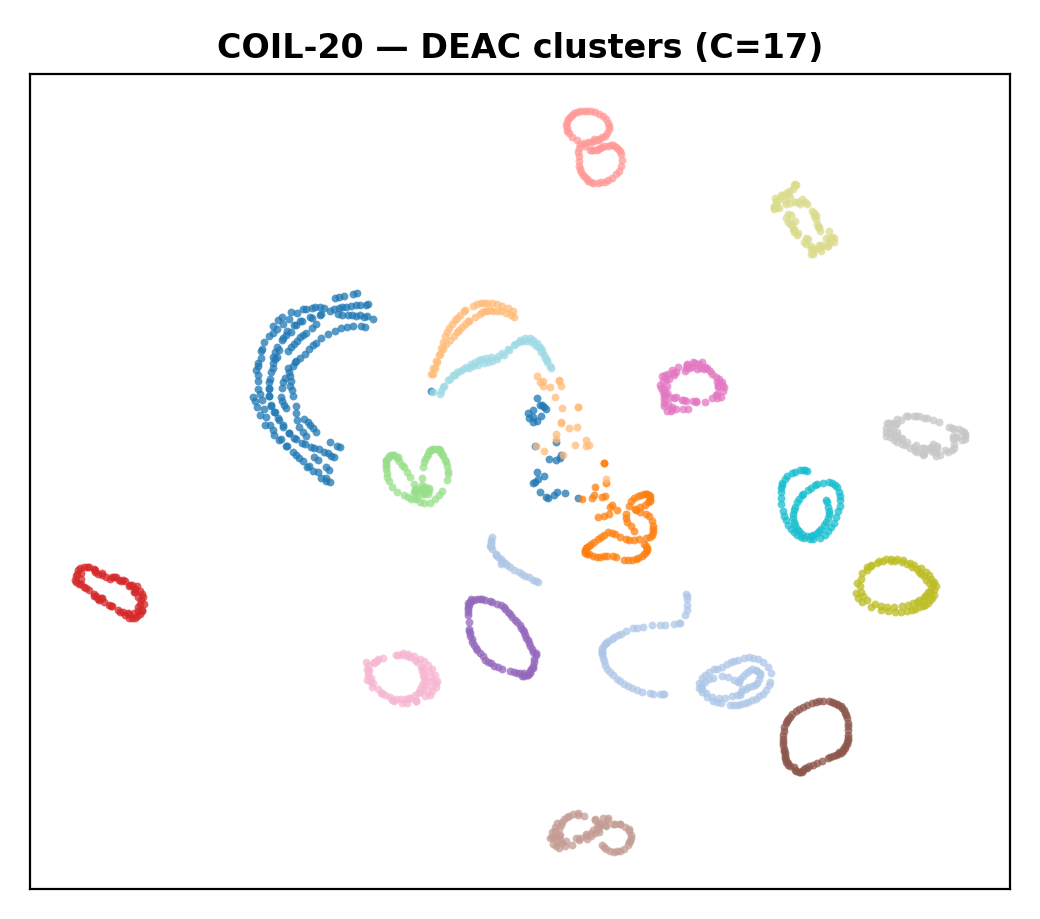
\includegraphics[width=0.225\textwidth]{figures/COIL20/tsne_COIL20.png} &
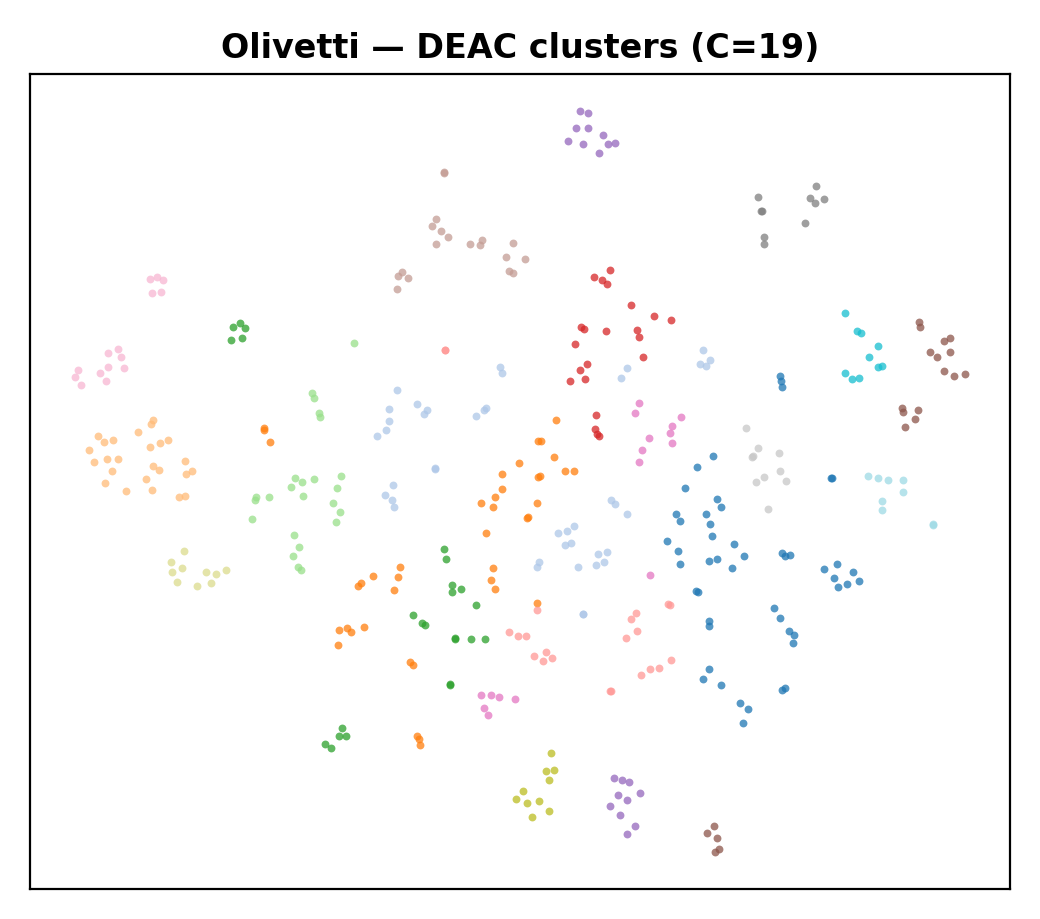
\includegraphics[width=0.225\textwidth]{figures/Olivetti/tsne_Olivetti.png} &
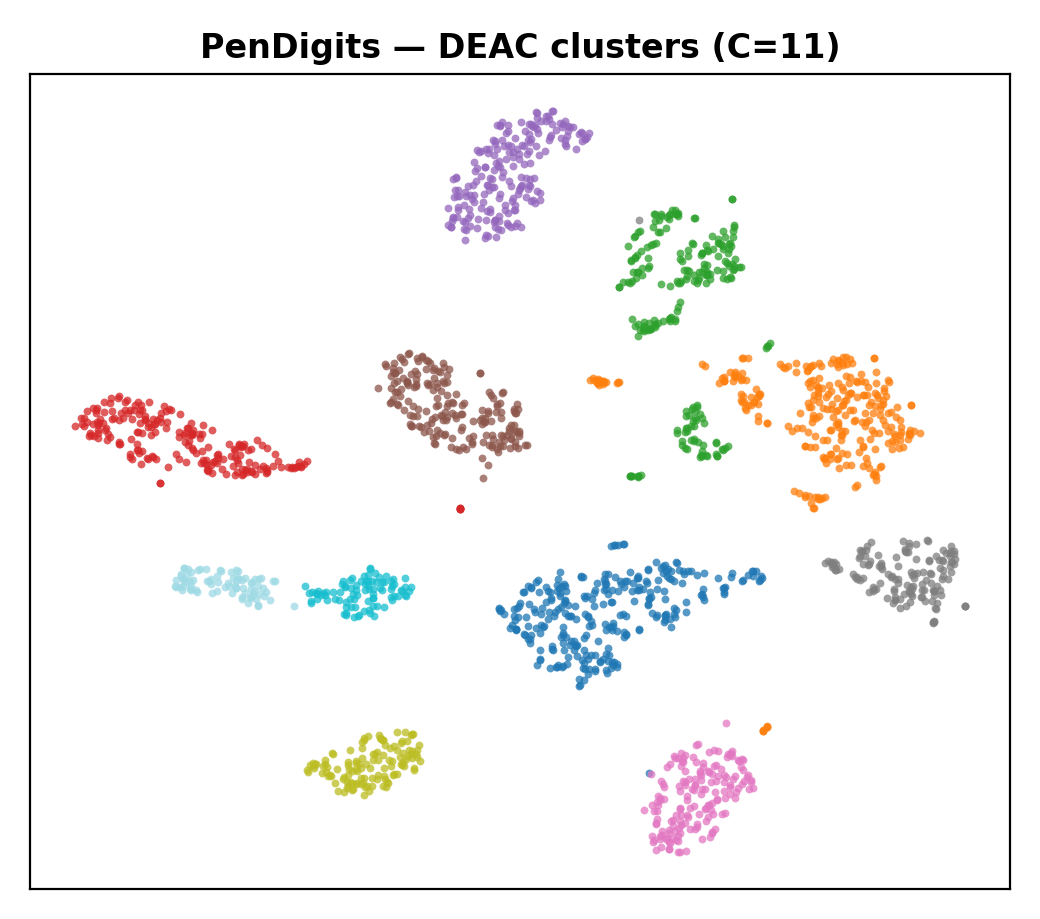
\includegraphics[width=0.225\textwidth]{figures/PenDigits/tsne_PenDigits.png} \\
\scriptsize (a) MFeat & \scriptsize (b) COIL-20 & \scriptsize (c) Olivetti & \scriptsize (d) PenDigits \\[3pt]
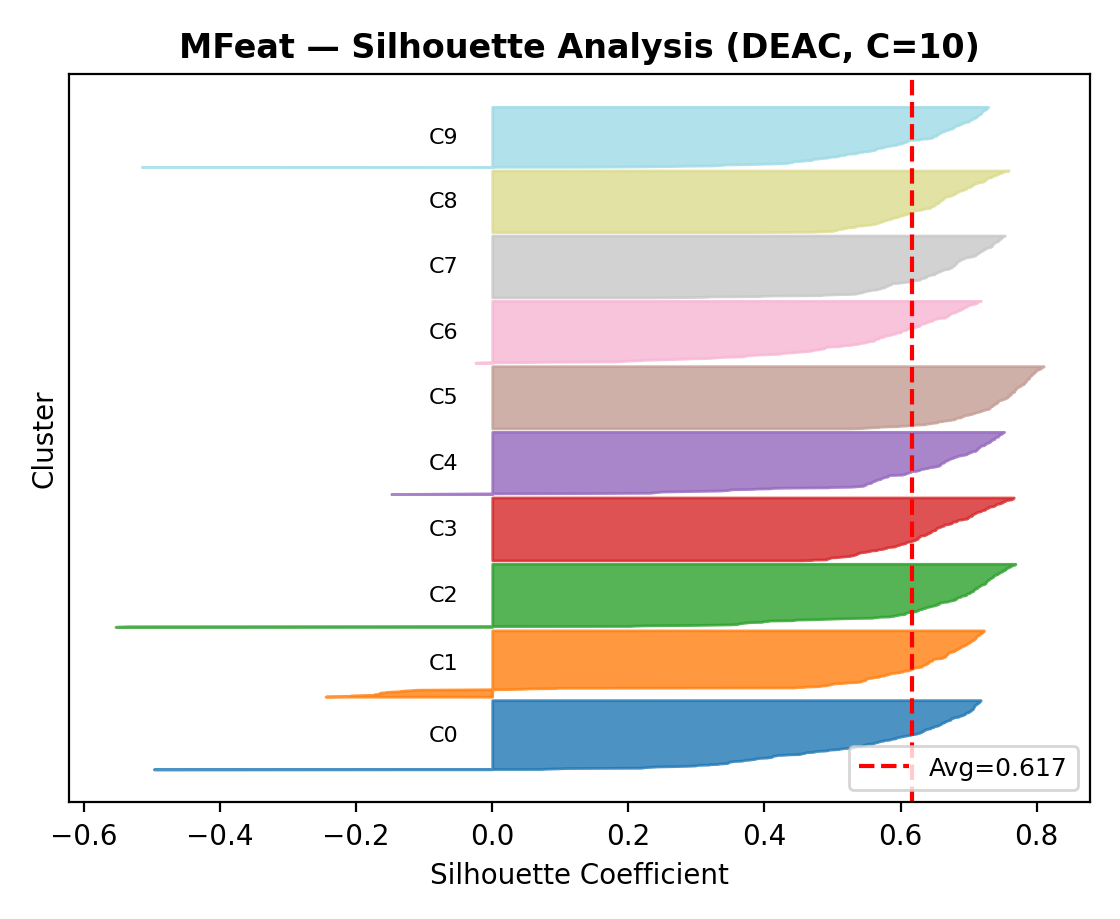
\includegraphics[width=0.225\textwidth]{figures/MFeat/silhouette_MFeat.png} &
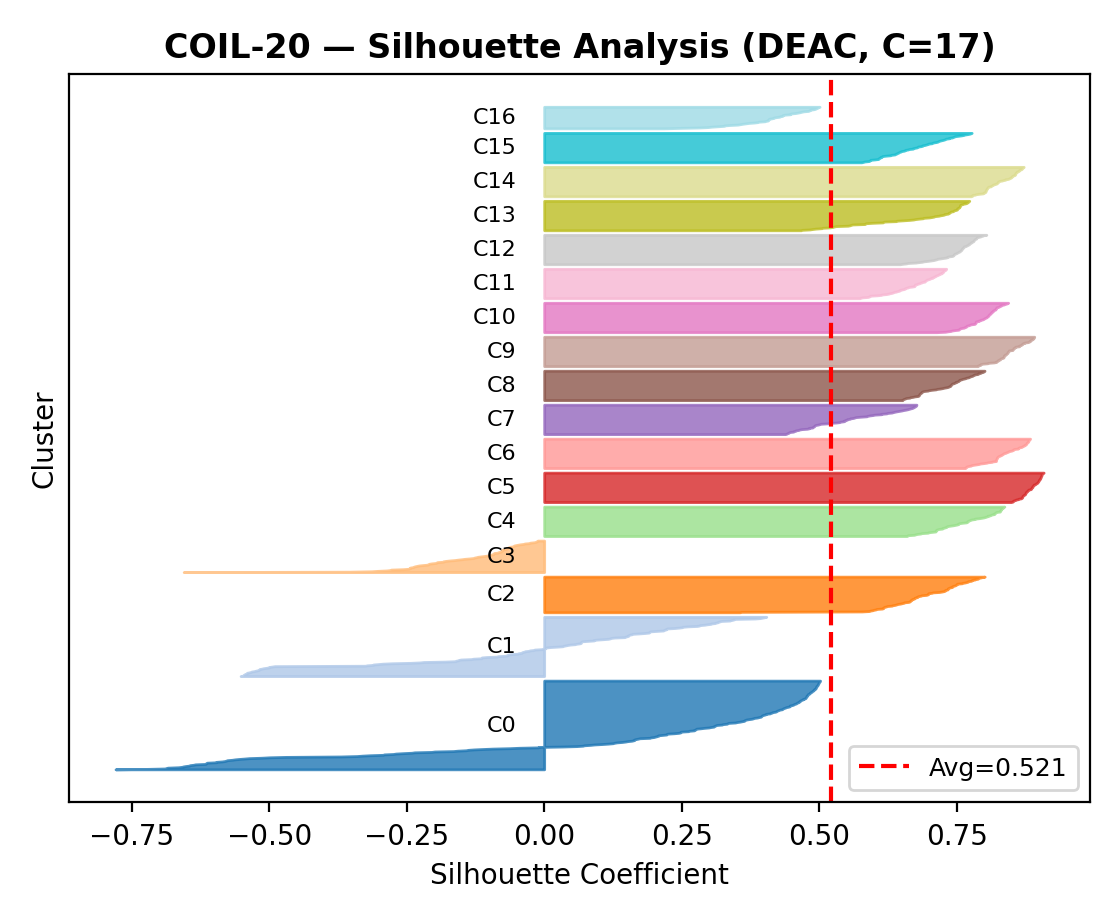
\includegraphics[width=0.225\textwidth]{figures/COIL20/silhouette_COIL20.png} &
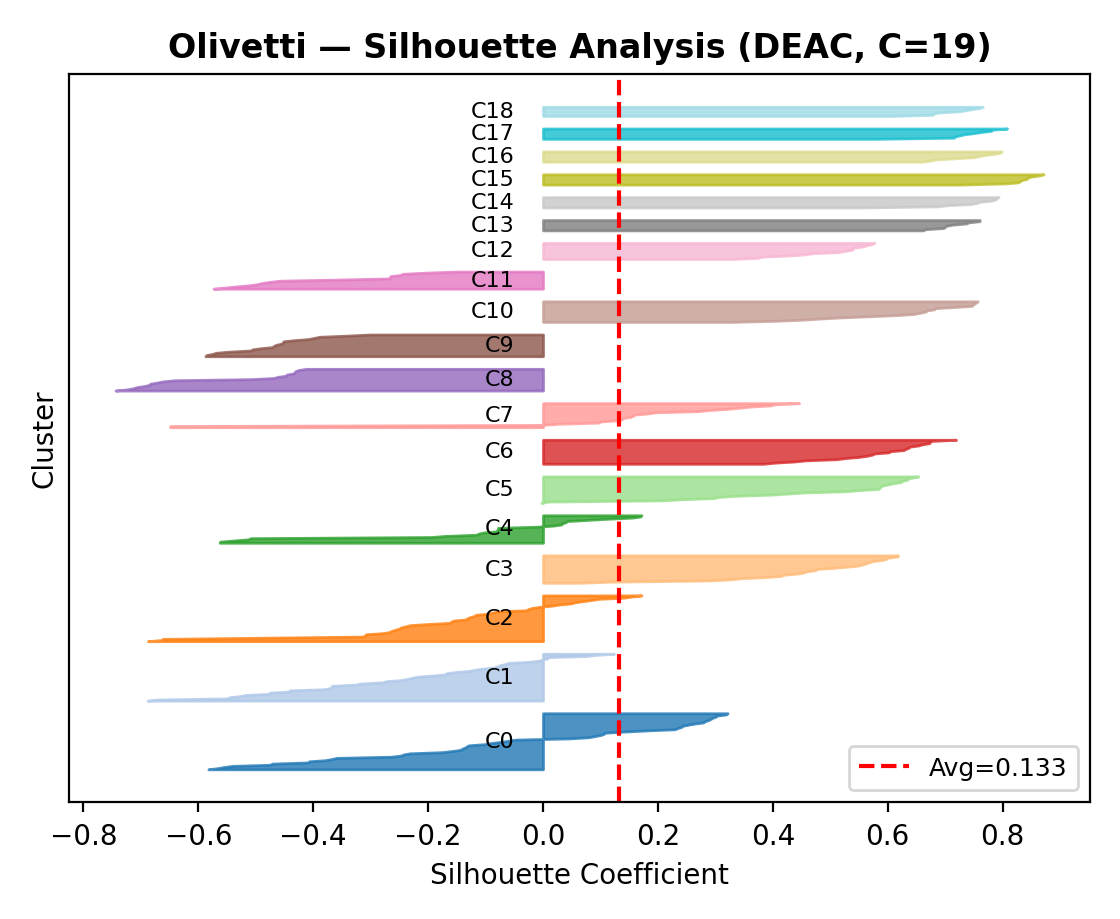
\includegraphics[width=0.225\textwidth]{figures/Olivetti/silhouette_Olivetti.png} &
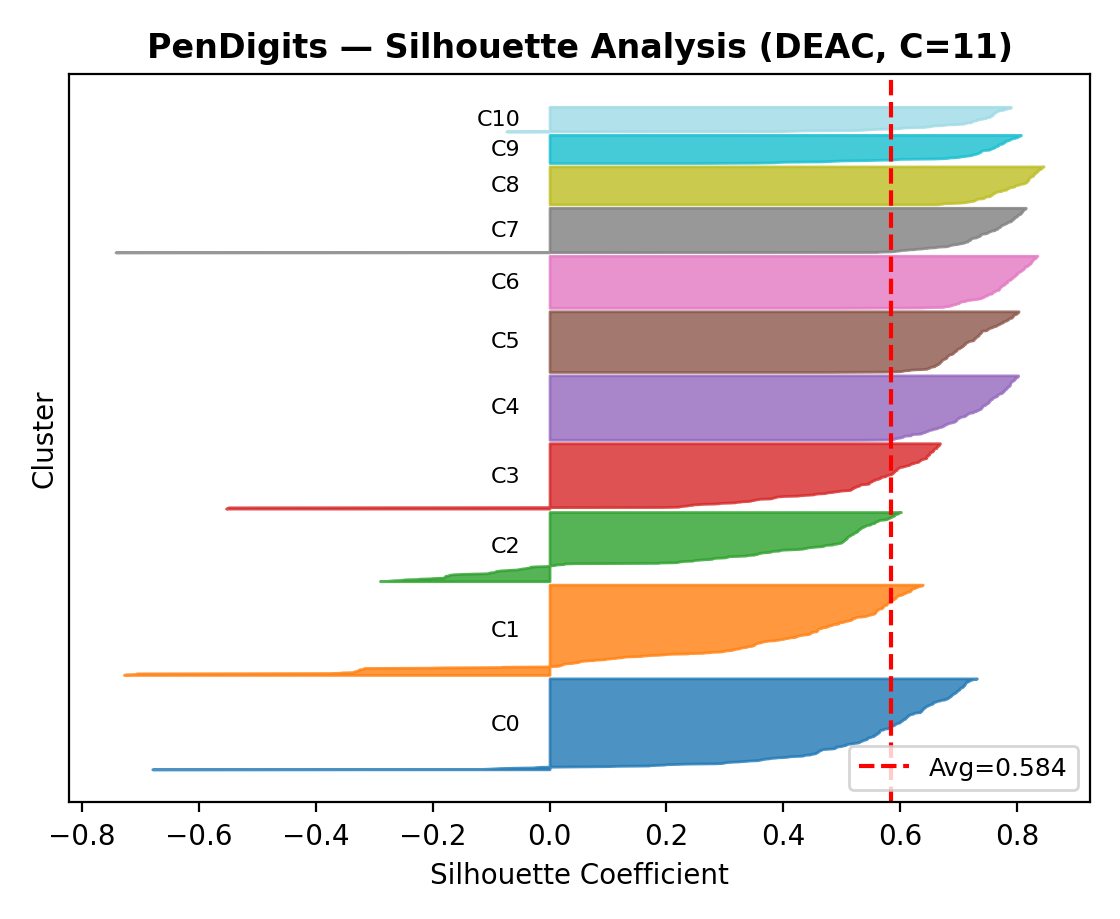
\includegraphics[width=0.225\textwidth]{figures/PenDigits/silhouette_PenDigits.png} \\
\scriptsize (e) MFeat sil. & \scriptsize (f) COIL-20 sil. & \scriptsize (g) Olivetti sil. & \scriptsize (h) PenDigits sil. \\
\end{tabular}
\caption{Qualitative analysis. Top~(a--d): t-SNE projections of DEAC clusters. Bottom~(e--h): silhouette plots.}
\label{fig:qualitative}
\end{figure*}

\subsection{Optimization Dynamics}

Fig.~\ref{fig:optim_dynamics} shows DE convergence curves and parameter exploration trajectories. Convergence occurs within 6--8 generations on most datasets. To separate the contribution of each component, we now ablate them.

\begin{figure}[!t]
\centering
\setlength{\tabcolsep}{2pt}
\begin{tabular}{cc}
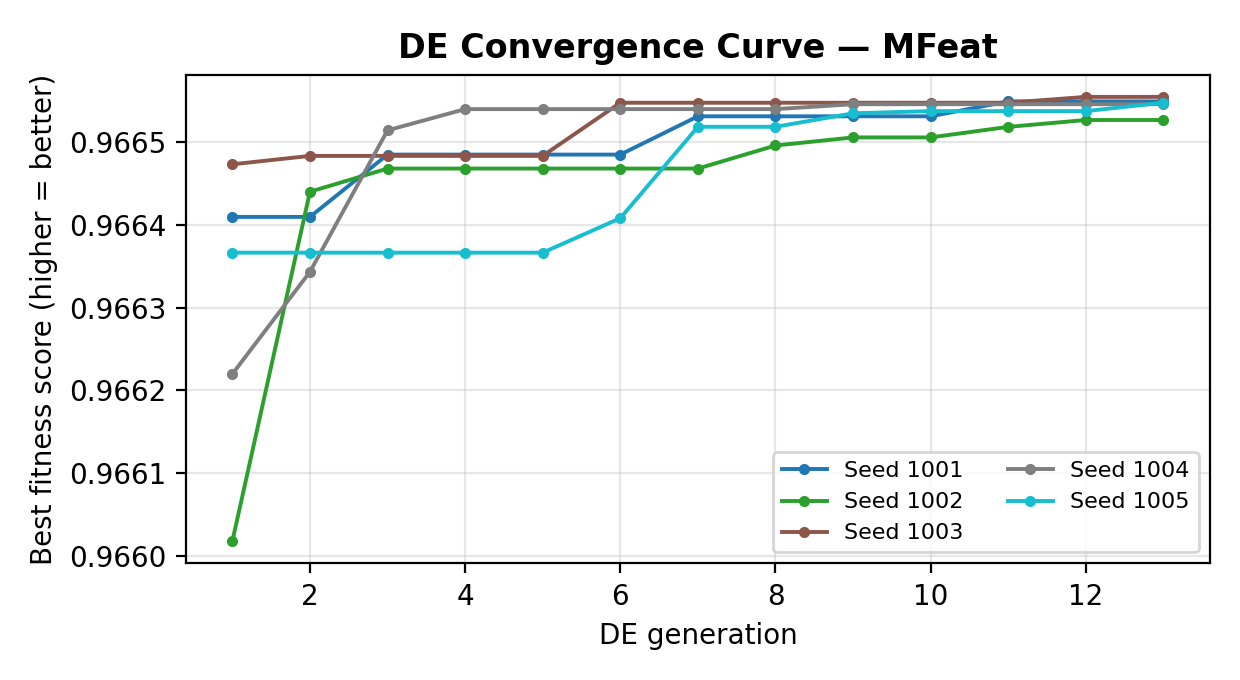
\includegraphics[width=0.45\columnwidth]{figures/MFeat/de_convergence_MFeat.png} &
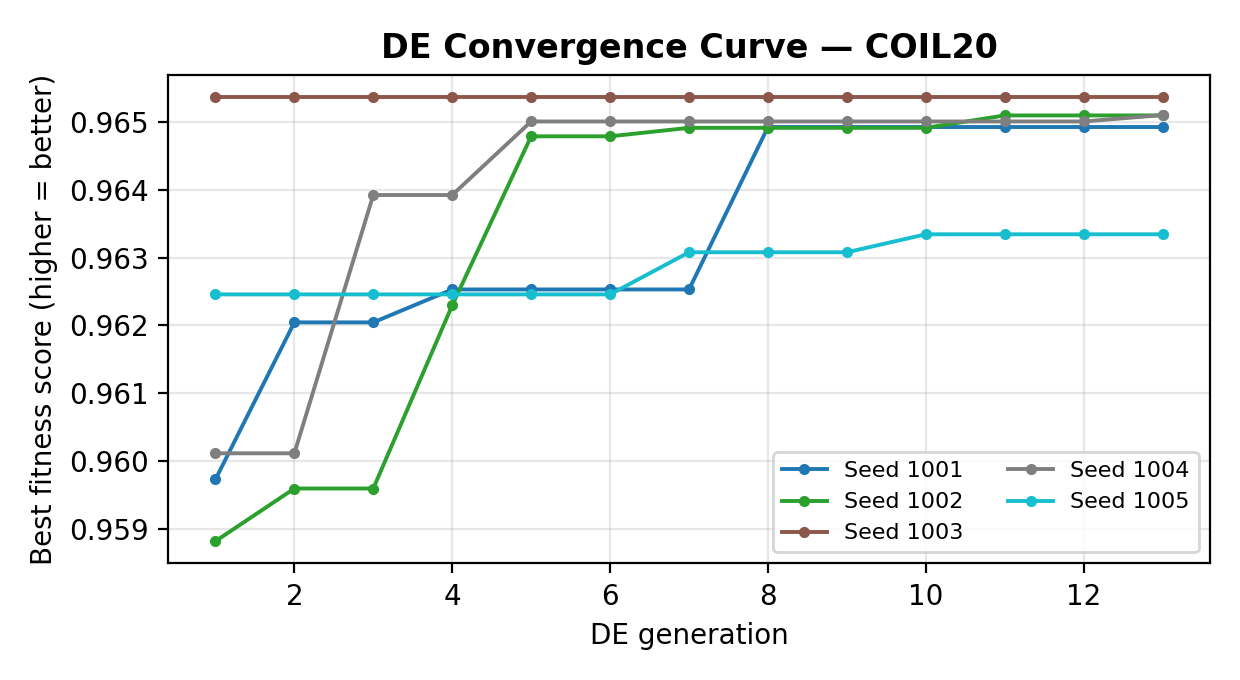
\includegraphics[width=0.45\columnwidth]{figures/COIL20/de_convergence_COIL20.png} \\
\scriptsize (a) Convergence --- MFeat & \scriptsize (b) Convergence --- COIL-20 \\[3pt]
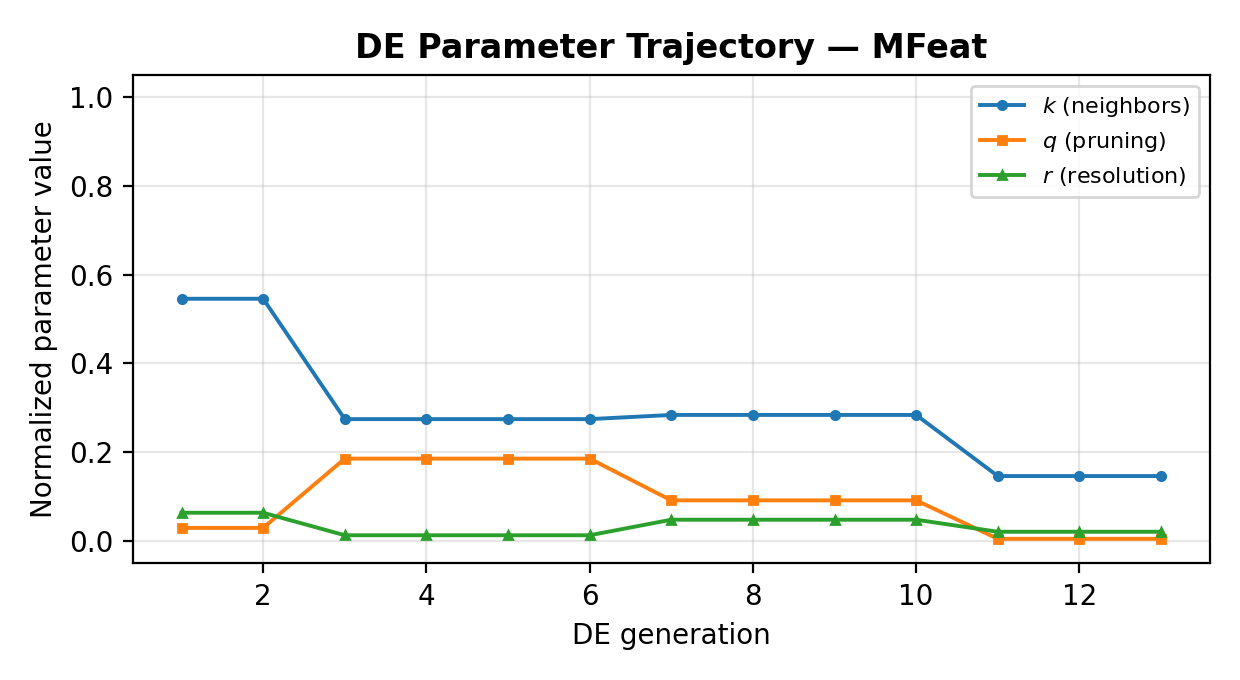
\includegraphics[width=0.45\columnwidth]{figures/MFeat/param_trajectory_MFeat.png} &
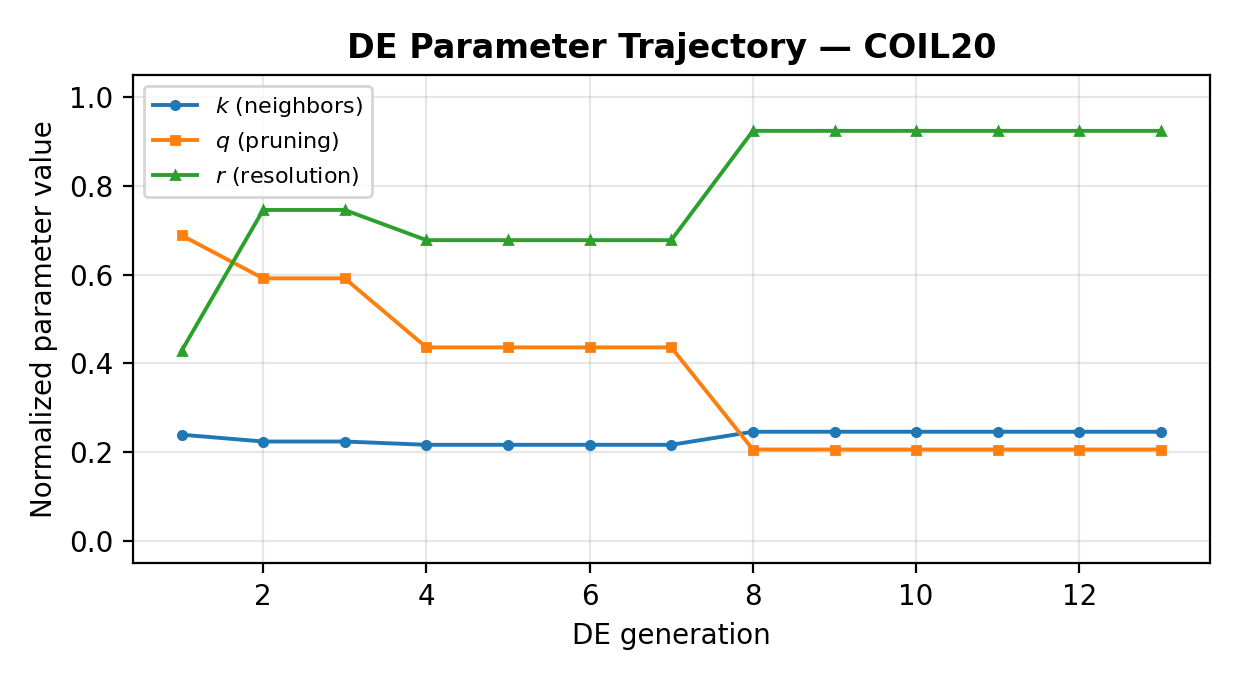
\includegraphics[width=0.45\columnwidth]{figures/COIL20/param_trajectory_COIL20.png} \\
\scriptsize (c) Trajectory --- MFeat & \scriptsize (d) Trajectory --- COIL-20 \\
\end{tabular}
\caption{DE optimization dynamics: convergence curves (top) and parameter trajectories (bottom).}
\label{fig:optim_dynamics}
\end{figure}

\subsection{Ablation Study}

Table~\ref{tab:ablation} isolates the contribution of every DEAC component.

\begin{table}[htbp]
\centering
\caption{Ablation study: mean ARI across 12 datasets under \emph{oracle} engine selection (upper bound; the deployable label-free gate is characterized in Table~\ref{tab:gate}).}
\label{tab:ablation}
\footnotesize
\begin{tabular}{lcc}
\toprule
Configuration & Mean ARI & $\Delta$ vs.\ PCA \\
\midrule
PCA Baseline (no optim.)           & 0.326 & --- \\
UMAP Baseline (no optim.)          & 0.574 & +75.8\% \\
PCA + DE                            & 0.504 & +54.6\% \\
UMAP + DE (AMR-DE)                 & 0.521 & +59.8\% \\
SNN + Leiden (EMR-CGC)             & 0.644 & +97.5\% \\
EMR-CGC + Baseline (oracle sel.)  & 0.646 & +98.2\% \\
\textbf{DEAC (full, +\,AMR-DE)}     & \textbf{0.649} & \textbf{+99.1\%} \\
\bottomrule
\end{tabular}
\end{table}

Four effects stand out. (i)~Switching from PCA to UMAP is the single largest
improvement (+75.8\%). (ii)~Adding SNN+Leiden (EMR-CGC) gains another 0.070
in mean ARI over the UMAP baseline (0.644 vs.\ 0.574) and is the true
workhorse of the framework.
(iii)~The optimization engine AMR-DE, used alone, is \emph{below} the UMAP
baseline (0.521 vs.\ 0.574)---a direct consequence of the internal--external
misalignment discussed in \S\ref{sec:disc}. (iv)~We report the marginal value
of AMR-DE honestly: over an ensemble-plus-baseline oracle (0.646), the
optimization engine adds only $+0.003$ mean ARI (0.649), and it is the
deciding output on just 2 of 12 datasets (COIL-20, ISOLET). Its contribution
is therefore narrow; the framework's strength comes from the ensemble and the
gate, with AMR-DE supplying complementary coverage where parameter search
helps. Fig.~\ref{fig:phase_waterfall} stacks these increments as a waterfall,
running from the PCA baseline to the full DEAC configuration. Accuracy gains
are only useful if the method remains affordable.

\begin{figure}[!t]
\centering
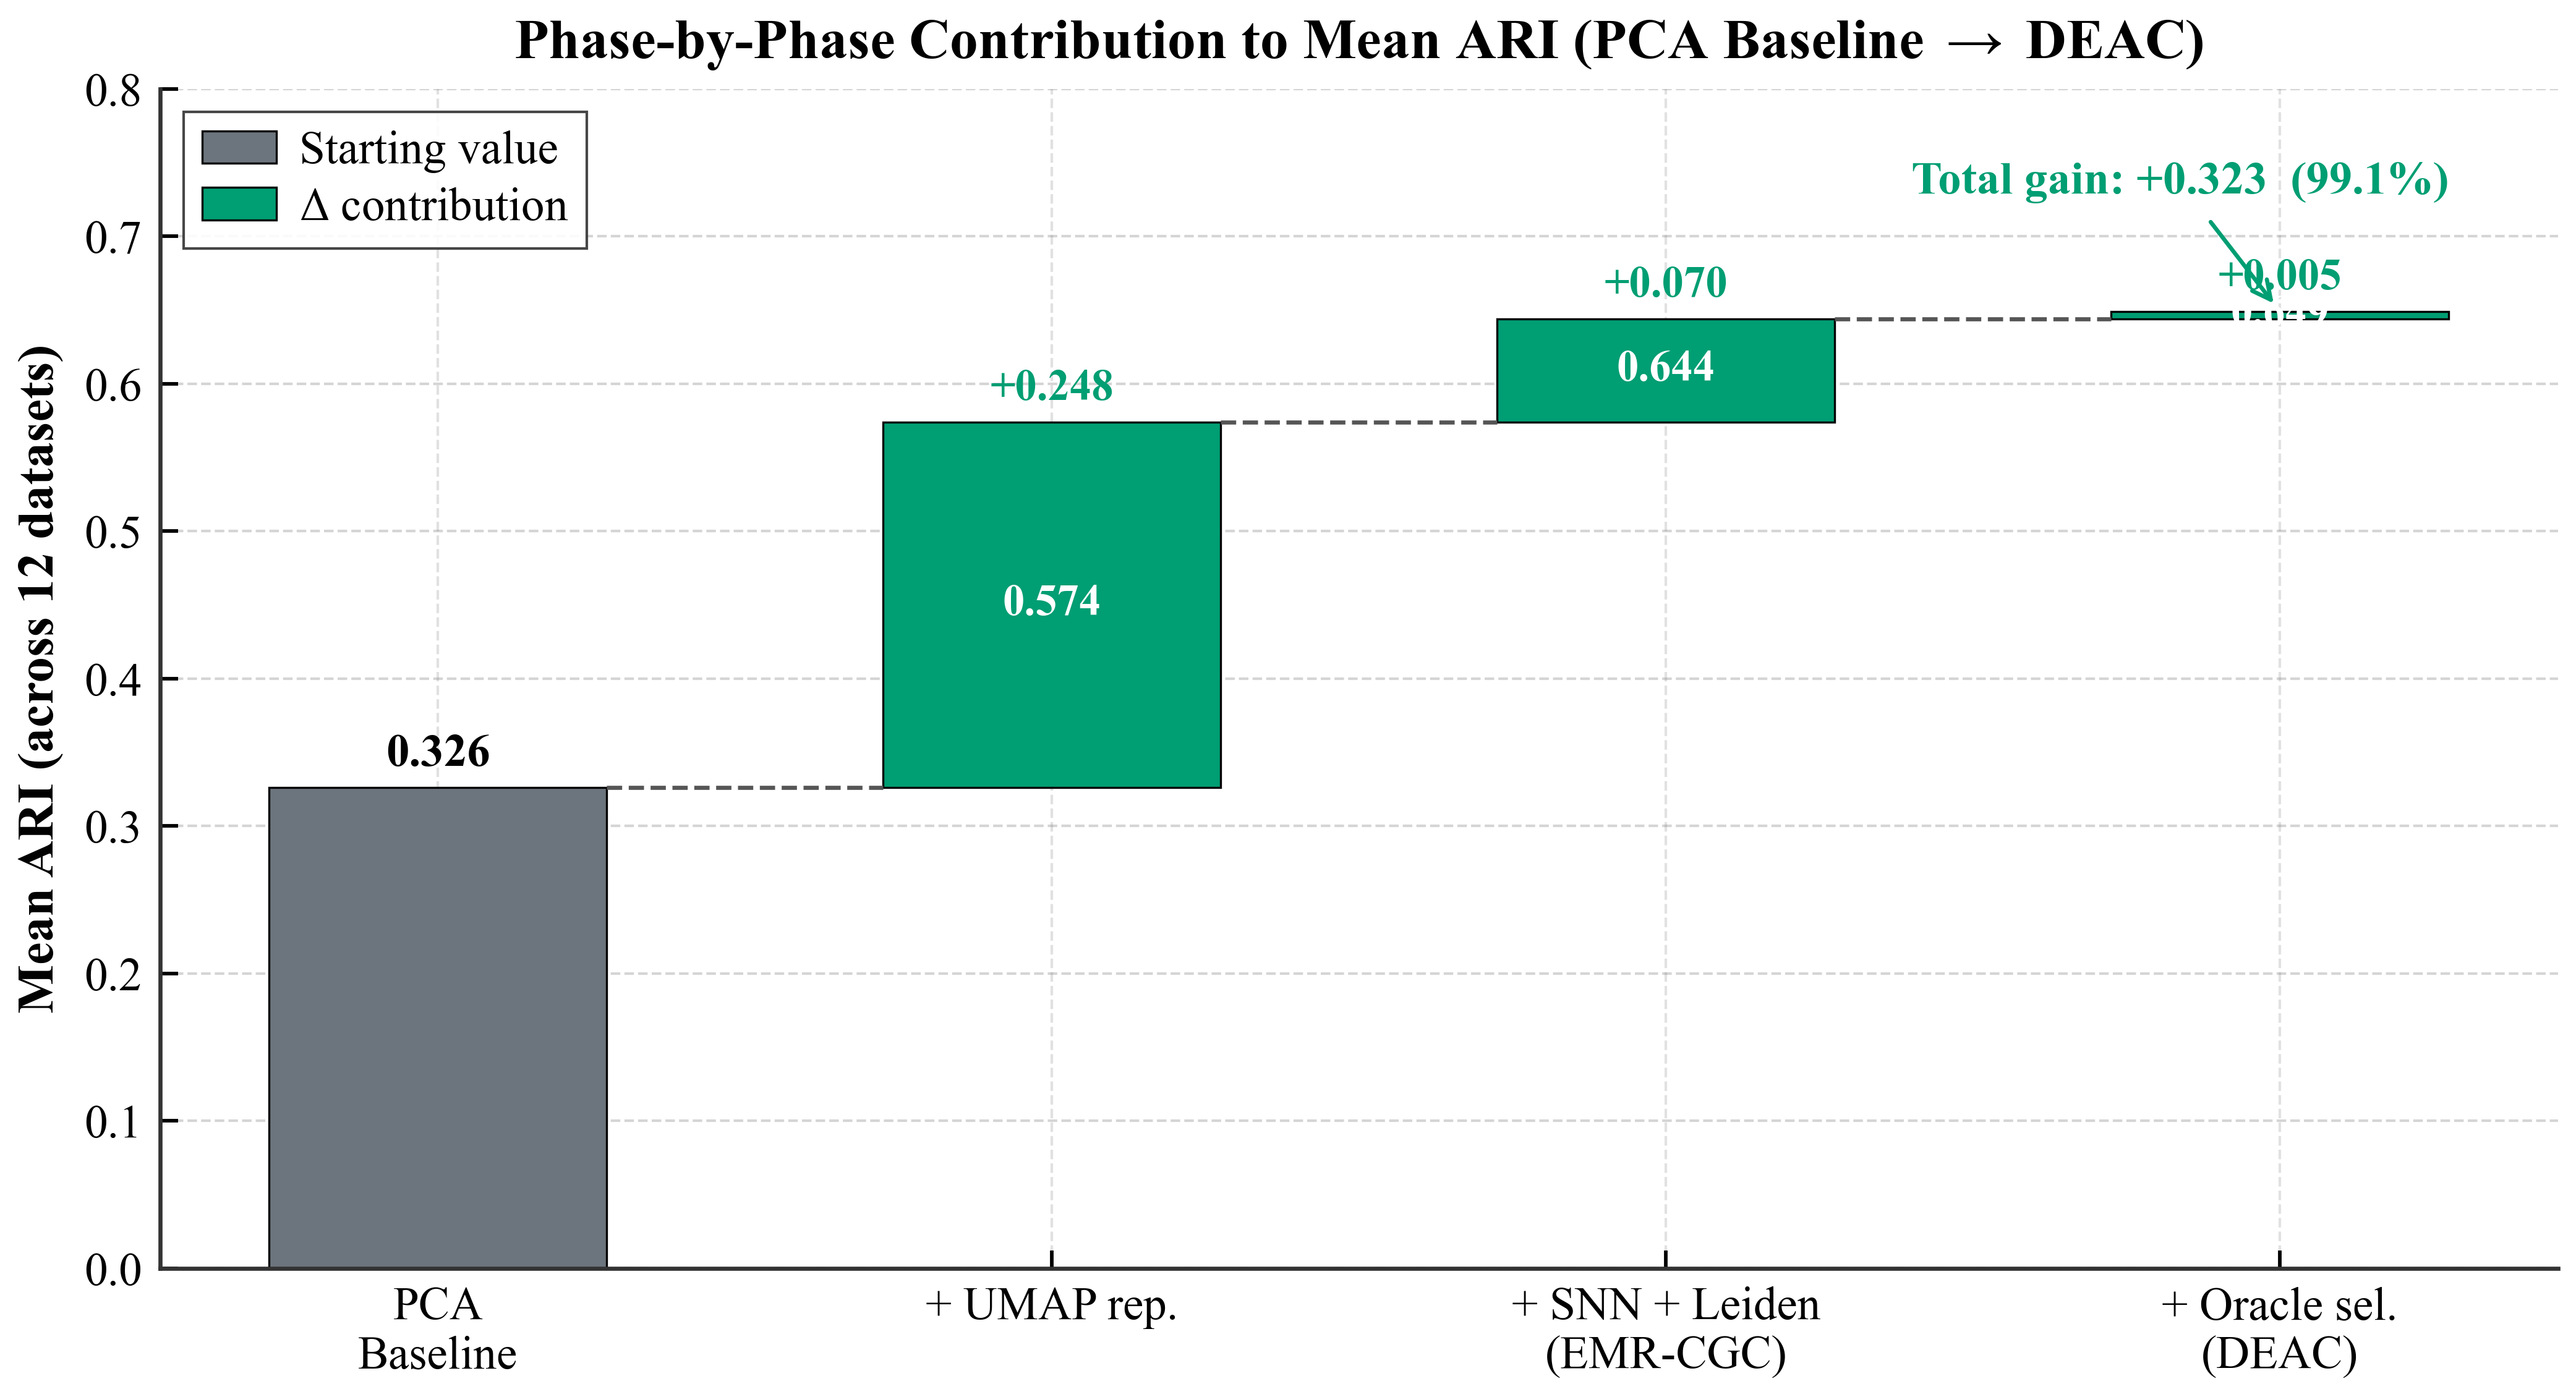
\includegraphics[width=0.95\columnwidth]{figures/cross_dataset/phase_waterfall.png}
\caption{Phase-by-phase contribution to mean ARI, averaged over 12 datasets. Starting from the PCA baseline (0.326), UMAP representation adds +0.248, SNN with Leiden community detection adds +0.070, and oracle engine selection adds +0.005 (an upper bound; the deployable label-free gate is characterized in Table~\ref{tab:gate}), for a DEAC mean ARI of 0.649---a total gain of 99.1\,\% over the PCA baseline.}
\label{fig:phase_waterfall}
\end{figure}

\subsection{Computational Complexity}

Table~\ref{tab:complexity} summarizes the theoretical cost of each component.

\begin{table}[htbp]
\centering
\caption{Computational complexity of DEAC components.}
\label{tab:complexity}
\footnotesize
\setlength{\tabcolsep}{3pt}
\begin{tabular}{lcc}
\toprule
Component & Complexity & Typical Cost \\
\midrule
StandardScaler        & $\mathcal{O}(nd)$                   & linear \\
PCA                   & $\mathcal{O}(nd \cdot d')$          & $\mathcal{O}(nd \cdot 40)$ \\
UMAP                  & $\mathcal{O}(n^{1.14} d')$          & near-linear \\
t-SNE                 & $\mathcal{O}(n^2)$                  & quadratic \\
KNN graph             & $\mathcal{O}(nk \cdot d')$          & $\mathcal{O}(nk \cdot 40)$ \\
SNN graph             & $\mathcal{O}(nk^2)$                 & $\mathcal{O}(n \cdot k^2)$ \\
Leiden                & $\mathcal{O}(m \log n)$             & near-linear \\
AMR-DE (all evals)    & $\mathcal{O}(E \cdot F_c)$          & $E{\approx}200$ \\
EMR-CGC ensemble      & $\mathcal{O}(M|K||R| F_c)$          & $60 \cdot F_c$ \\
\midrule
\textbf{Total DEAC}   & $\mathcal{O}(n^{1.14} d' + n k^2)$  & sub-quadratic \\
\bottomrule
\end{tabular}
\end{table}

Measured end-to-end runtimes on an Intel~i7 CPU---Wine (178) 14\,s, MFeat (2000) 24\,s, USPS (9298) 45\,s---keep runtime practical even at the high end of our benchmarks.

% ============================================================
% 5. DISCUSSION
% ============================================================
\section{Discussion}\label{sec:disc}

The results raise four follow-up questions: why arbitration rather than optimization, how much of the oracle a label-free gate can recover, why SNN rather than KNN, and where the method still falls short.

\subsection{Why Arbitration, Not Optimization?}

The most informative result in our study is a negative one. AMR-DE
explicitly maximizes internal objectives (modularity, silhouette,
Calinski--Harabasz), yet its mean ARI (0.521) falls \emph{below} the fixed
baseline (0.574) and it collapses outright on several datasets
(Segmentation 0.169, Satimage 0.277, USPS 0.533). Internal quality and
external agreement are therefore misaligned: a partition can be ``better''
by every internal score and worse by ARI. This is precisely why DEAC does
not trust any single optimized candidate. The QualityGate instead
\emph{arbitrates}: it keeps the optimization-based output only when it
survives three conservative tests, and otherwise falls back to the
ensemble or the baseline. The benefit of the optimization engine is thus
narrow but real---it is the deciding output on only COIL-20 and ISOLET
(well-separated, moderate-$C$ data where parameter search pays off),
contributing $+0.003$ to the mean ARI over an ensemble-plus-baseline system
(0.646 $\to$ 0.649). We report this small margin openly: AMR-DE is a
complementary engine for specific regimes, not the workhorse. The workhorse
is EMR-CGC (0.644), and the safety net is the gate---but that gate must choose
without labels, which raises the question of how much of the label-aware oracle
it can actually recover.

\subsection{How Much of the Oracle Is Deployable?}

The main results (Table~\ref{tab:main_results}) select the best engine per dataset using ground-truth ARI---an oracle unavailable at deployment, where the QualityGate must choose from internal metrics alone. Table~\ref{tab:gate} quantifies the gap on the full data with our exact pipeline at a single seed; its absolute ARIs therefore differ marginally from the five-seed main tables (baseline $0.582$ vs.\ $0.574$), but the gap---not the absolute level---is the quantity of interest. The deployable gate reaches a mean ARI of $0.630$ against the oracle's $0.646$ and the baseline's $0.582$, recovering $75\%$ of the oracle's gain and agreeing with the oracle's engine choice on $6$ of $12$ datasets. The residual gap is a direct expression of the internal--external misalignment that motivates this work: the gate errs precisely where an engine is best by ARI but not by internal score, most visibly on ISOLET (where AMR-DE is secretly optimal) and Olivetti (where EMR-CGC is). The same mechanism means the gate is not strictly monotone over the baseline---on Wine it prefers AMR-DE on internal grounds and loses $0.028$ ARI. We therefore treat the oracle as an upper bound and the gate as the honest deployable performance, and regard closing their gap---better internal proxies for external quality---as the central open problem. The gate's ingredients invite the same scrutiny, beginning with the SNN graph on which EMR-CGC is built.

% Auto-generated by build_gate_oracle.py
\begin{table}[!t]
\centering
\caption{Deployable QualityGate (selects among the three engines by internal metrics, \emph{no labels}) vs.\ the oracle upper bound (best-ARI engine per dataset). Full data, single seed with our exact pipeline, so absolute ARIs differ marginally from the five-seed main tables. $\Delta$ is oracle$-$gate.}
\label{tab:gate}
\footnotesize
\setlength{\tabcolsep}{4pt}
\begin{tabular}{lccc c}
\toprule
Dataset & Gate pick & Gate ARI & Oracle ARI & $\Delta$ \\
\midrule
Wine & AMR-DE & 0.774 & 0.802 & +0.028 \\
Glass & EMR & 0.164 & 0.171 & +0.007 \\
Olivetti & AMR-DE & 0.229 & 0.302 & +0.073 \\
CNAE-9 & Base & $\mathbf{0.637}$ & 0.637 & +0.000 \\
COIL-20 & EMR & 0.776 & 0.819 & +0.043 \\
Optdigits & AMR-DE & 0.848 & 0.849 & +0.001 \\
MFeat & EMR & $\mathbf{0.939}$ & 0.939 & +0.000 \\
Segmentation & Base & $\mathbf{0.443}$ & 0.443 & +0.000 \\
ISOLET & EMR & 0.477 & 0.518 & +0.041 \\
Satimage & EMR & $\mathbf{0.600}$ & 0.600 & +0.000 \\
USPS & EMR & $\mathbf{0.922}$ & 0.922 & +0.000 \\
PenDigits & EMR & $\mathbf{0.751}$ & 0.751 & +0.000 \\
\midrule
\textbf{Mean} & --- & \textbf{0.630} & 0.646 & +0.016 \\
\bottomrule
\end{tabular}
\end{table}

\subsection{SNN vs.\ KNN Graph Construction}

SNN weighting is not a uniform win, and it is worth being precise about where it helps. Under a matched single-graph protocol (same UMAP representation, $k{=}35$, $r{=}0.25$), swapping KNN+Louvain for SNN+Leiden changes mean ARI only marginally---from 0.580 to 0.568, a $1.2$-point decrease on average. The average, however, hides a clear pattern that follows the theory of \S\ref{sec:rationale}: SNN improves precisely on the \emph{high-dimensional} datasets, where distance concentration degrades raw-distance weights---Olivetti ($d{=}4096$, $+0.027$), CNAE-9 ($d{=}856$, $+0.028$), and COIL-20 ($d{=}1024$, $+0.038$)---while it costs accuracy on lower-dimensional inputs (USPS $-0.076$, PenDigits $-0.058$). SNN is therefore a targeted tool for high-dimensional regimes, not a blanket improvement, and EMR-CGC's overall gain comes primarily from \emph{ensemble diversity} (five representations $\times$ twelve configurations with best-run selection) rather than from the SNN weighting alone. Neither choice removes every limitation, which we list next.

\subsection{Limitations}

(i)~\emph{Runtime.} EMR-CGC's 60-run ensemble is costlier than single-shot methods, though it stays under 60\,s per dataset in our experiments.
(ii)~\emph{Internal--external gap.} The QualityGate decides on internal metrics (MOD, SIL, BAL), which do not align perfectly with ARI, so the deployable gate is not strictly monotone over the baseline---on Wine it prefers AMR-DE on internal grounds and loses $0.028$ ARI (Table~\ref{tab:gate}).
(iii)~\emph{Scalability.} SNN is $\mathcal{O}(n k^2)$, so very large $n$ ($>50{,}000$) would require approximate-NN construction.
(iv)~\emph{Oracle vs.\ deployable gap.} The main-table DEAC is an oracle upper bound; the deployable label-free gate recovers $75\%$ of its gain over the baseline and sits modestly below N2D (Table~\ref{tab:gate}). Closing this gap with better internal proxies for external quality---or a learned representation in the RepScan stage---is the primary open problem.

% ============================================================
% 6. CONCLUSION
% ============================================================
\section{Conclusion}\label{sec:conc}

We presented DEAC (Defensive Ensemble Adaptive Clustering), a framework for graph-based clustering of high-dimensional data that infers the cluster count rather than requiring it. Its core is a multi-representation SNN--Leiden ensemble (EMR-CGC) arbitrated by a three-layer QualityGate, with a complementary DE-optimized engine (AMR-DE) that contributes on specific regimes. The design is motivated by a negative result---optimizing internal metrics can degrade external accuracy---against which the gate is built to defend. DEAC lifts mean ARI by 13.1\% over the baseline across 12 benchmarks; when every method must discover $C$, it significantly outperforms five classical methods on 9 of 12 datasets (Holm-corrected Wilcoxon, Friedman $p{<}0.001$); and an oracle over its engines matches the strongest deep-clustering method (N2D) while inferring the cluster count that N2D is given, with the deployable label-free gate recovering $75\%$ of that oracle's gain. Three extensions remain open.

The first is approximate-NN SNN construction, which would extend DEAC beyond $n{=}50$k. The second is integrating deep representation learning into the RepScan stage. The third is a semi-supervised variant that uses partial labels to close the internal--external metric gap identified in \S\ref{sec:disc}.

\vspace{2pt}
\noindent\textit{Code and data availability.} The framework, all experiment scripts, and the oracle--deployable gap study are available at \url{https://github.com/al-shaibani-star/-DEAC}.

% ============================================================
% REFERENCES
% ============================================================
\begin{thebibliography}{30}

\bibitem{jain2010data}
A.~K.~Jain, ``Data clustering: 50 years beyond K-means,'' \emph{Pattern Recognition Letters}, vol.~31, no.~8, pp.~573--580, 2010.

\bibitem{steinbach2004challenges}
M.~Steinbach, L.~Ert\"{o}z, and V.~Kumar, ``The challenges of clustering high dimensional data,'' in \emph{New Directions in Statistical Physics}, Springer, 2004, pp.~273--309.

\bibitem{lloyd1982least}
S.~Lloyd, ``Least squares quantization in PCM,'' \emph{IEEE Trans.\ Inf.\ Theory}, vol.~28, no.~2, pp.~129--137, 1982.

\bibitem{ng2001spectral}
A.~Y.~Ng, M.~I.~Jordan, and Y.~Weiss, ``On spectral clustering: Analysis and an algorithm,'' in \emph{Proc.\ NeurIPS}, 2001, pp.~849--856.

\bibitem{campello2013density}
R.~J.~G.~B.~Campello, D.~Moulavi, and J.~Sander, ``Density-based clustering based on hierarchical density estimates,'' in \emph{Proc.\ PAKDD}, Springer, 2013, pp.~160--172.

\bibitem{schaeffer2007graph}
S.~E.~Schaeffer, ``Graph clustering,'' \emph{Computer Science Review}, vol.~1, no.~1, pp.~27--64, 2007.

\bibitem{blondel2008fast}
V.~D.~Blondel, J.-L.~Guillaume, R.~Lambiotte, and E.~Lefebvre, ``Fast unfolding of communities in large networks,'' \emph{J.\ Stat.\ Mech.}, vol.~2008, no.~10, p.~P10008, 2008.

\bibitem{traag2019louvain}
V.~A.~Traag, L.~Waltman, and N.~J.~van~Eck, ``From Louvain to Leiden: guaranteeing well-connected communities,'' \emph{Scientific Reports}, vol.~9, no.~1, p.~5233, 2019.

\bibitem{jolliffe2002principal}
I.~T.~Jolliffe, \emph{Principal Component Analysis}, 2nd~ed. Springer, 2002.

\bibitem{mcinnes2018umap}
L.~McInnes, J.~Healy, and J.~Melville, ``UMAP: Uniform Manifold Approximation and Projection for dimension reduction,'' \emph{arXiv:1802.03426}, 2018.

\bibitem{van2008visualizing}
L.~van~der~Maaten and G.~Hinton, ``Visualizing data using t-SNE,'' \emph{J.\ Mach.\ Learn.\ Res.}, vol.~9, pp.~2579--2605, 2008.

\bibitem{storn1997differential}
R.~Storn and K.~Price, ``Differential evolution---a simple and efficient heuristic for global optimization over continuous spaces,'' \emph{J.\ Global Optim.}, vol.~11, no.~4, pp.~341--359, 1997.

\bibitem{mirjalili2014grey}
S.~Mirjalili, S.~M.~Mirjalili, and A.~Lewis, ``Grey Wolf Optimizer,'' \emph{Advances in Engineering Software}, vol.~69, pp.~46--61, 2014.

\bibitem{yang2010nature}
X.-S.~Yang, \emph{Nature-Inspired Metaheuristic Algorithms}, 2nd~ed. Luniver Press, 2010.

\bibitem{faris2018grey}
H.~Faris, I.~Aljarah, M.~A.~Al-Betar, and S.~Mirjalili, ``Grey wolf optimizer: a review of recent variants and applications,'' \emph{Neural Computing and Applications}, vol.~30, no.~2, pp.~413--435, 2018.

\bibitem{ertoz2003finding}
L.~Ert\"{o}z, M.~Steinbach, and V.~Kumar, ``Finding clusters of different sizes, shapes, and densities in noisy, high dimensional data,'' in \emph{Proc.\ SIAM Int.\ Conf.\ Data Mining}, 2003, pp.~47--58.

\bibitem{wang2026density}
Y.~Wang and M.~J.~Samonte, ``Density peak clustering algorithm based on adaptive K-nearest neighbors for manifold data,'' \emph{Discover Applied Sciences}, vol.~8, art.~165, 2026.

\bibitem{strehl2002cluster}
A.~Strehl and J.~Ghosh, ``Cluster ensembles---a knowledge reuse framework for combining multiple partitions,'' \emph{J.\ Mach.\ Learn.\ Res.}, vol.~3, pp.~583--617, 2002.

\bibitem{fred2005combining}
A.~L.~N.~Fred and A.~K.~Jain, ``Combining multiple clusterings using evidence accumulation,'' \emph{IEEE Trans.\ Pattern Anal.\ Mach.\ Intell.}, vol.~27, no.~6, pp.~835--850, 2005.

\bibitem{vega2011survey}
S.~Vega-Pons and J.~Ruiz-Shulcloper, ``A survey of clustering ensemble algorithms,'' \emph{Int.\ J.\ Pattern Recognit.\ Artif.\ Intell.}, vol.~25, no.~3, pp.~337--372, 2011.

\bibitem{hubert1985comparing}
L.~Hubert and P.~Arabie, ``Comparing partitions,'' \emph{J.\ Classification}, vol.~2, no.~1, pp.~193--218, 1985.

\bibitem{yang2010image}
Y.~Yang, D.~Xu, F.~Nie, S.~Yan, and Y.~Zhuang, ``Image clustering using local discriminant models and global integration,'' \emph{IEEE Trans.\ Image Process.}, vol.~19, no.~10, pp.~2761--2773, 2010.

\bibitem{das2008automatic}
S.~Das, A.~Abraham, and A.~Konar, ``Automatic clustering using an improved differential evolution algorithm,'' \emph{IEEE Trans.\ Syst., Man, Cybern.\ A}, vol.~38, no.~1, pp.~218--237, 2008.

\bibitem{becht2019dimensionality}
E.~Becht \emph{et al.}, ``Dimensionality reduction for visualizing single-cell data using UMAP,'' \emph{Nature Biotechnology}, vol.~37, pp.~38--44, 2019.

\bibitem{brito1997connectivity}
M.~R.~Brito, E.~L.~Ch\'{a}vez, A.~J.~Quiroz, and J.~E.~Yukich, ``Connectivity of the mutual $k$-nearest-neighbor graph in clustering and outlier detection,'' \emph{Statistics \& Probability Letters}, vol.~35, no.~1, pp.~33--42, 1997.

\bibitem{satuluri2011local}
V.~Satuluri, S.~Parthasarathy, and D.~Ruan, ``Local graph sparsification for scalable clustering,'' in \emph{Proc.\ ACM SIGMOD}, 2011, pp.~721--732.

\bibitem{xie2016unsupervised}
J.~Xie, R.~Girshick, and A.~Farhadi, ``Unsupervised deep embedding for clustering analysis,'' in \emph{Proc.\ ICML}, 2016, pp.~478--487.

\bibitem{mcconville2021n2d}
R.~McConville, R.~Santos-Rodriguez, R.~J.~Piechocki, and I.~Craddock, ``N2D: (Not too) deep clustering via clustering the local manifold of an autoencoded embedding,'' in \emph{Proc.\ ICPR}, 2021, pp.~5145--5152.

\bibitem{guo2017improved}
X.~Guo, L.~Gao, X.~Liu, and J.~Yin, ``Improved deep embedded clustering with local structure preservation,'' in \emph{Proc.\ IJCAI}, 2017, pp.~1753--1759.

\bibitem{yang2017towards}
B.~Yang, X.~Fu, N.~D.~Sidiropoulos, and M.~Hong, ``Towards K-means-friendly spaces: Simultaneous deep learning and clustering,'' in \emph{Proc.\ ICML}, 2017, pp.~3861--3870.

\bibitem{mardia1979multivariate}
K.~V.~Mardia, J.~T.~Kent, and J.~M.~Bibby, \emph{Multivariate Analysis}. Academic Press, 1979.

\bibitem{beyer1999nearest}
K.~Beyer, J.~Goldstein, R.~Ramakrishnan, and U.~Shaft, ``When is ``nearest neighbor'' meaningful?'' in \emph{Proc.\ ICDT}, 1999, pp.~217--235.

\bibitem{houle2010shared}
M.~E.~Houle, H.-P.~Kriegel, P.~Kr\"{o}ger, E.~Schubert, and A.~Zimek, ``Can shared-neighbor distances defeat the curse of dimensionality?'' in \emph{Proc.\ SSDBM}, 2010, pp.~482--500.

\end{thebibliography}

\end{document}
